\documentclass[a4paper,11pt,twoside]{thesis}

\usepackage[british]{babel}
\usepackage{csquotes}
\usepackage{debug}
\usepackage{sciencestuff}
\usepackage{import}

\author{Riccardo Finotello}
\title{Theoretical and Computational Aspects of String Theory and Their Phenomenological Implications}
\advisor{Igor Pesando}
\institution{Università degli Studi di Torino}
\school{Scuola di Dottorato}
\specialisation{Dottorato in Fisica ed Astrofisica}
\logo{img/unito}

\addbibresource{thesis.bib}

\hypersetup{%
  pdfauthor={Riccardo Finotello}
}

%---- additional commands
\newcommand{\sm}{\textsc{sm}\xspace}
\newcommand{\eom}{\textsc{e.o.m.}\xspace}
\newcommand{\cft}{\textsc{cft}\xspace}
\newcommand{\ope}{\textsc{ope}\xspace}
\newcommand{\ap}{\ensuremath{\alpha'}}

%---- derivatives
\newcommand{\pd}{\ensuremath{\partial}}
\newcommand{\bpd}{\ensuremath{\overline{\partial}}}

%---- integrals
\newcommand{\ddz}{\ensuremath{\frac{\mathrm{d}z}{2 \pi i}}}
\newcommand{\ddbz}{\ensuremath{\frac{\mathrm{d}\overline{z}}{2 \pi i}}}
\newcommand{\cint}[1]{\ensuremath{\oint\limits_{\ccC_{#1}}}}

%---- operators
\newcommand{\bT}{\ensuremath{\overline{T}}}
\newcommand{\bL}{\ensuremath{\overline{L}}}

%---- states
\newcommand{\regvacuum}{\ensuremath{\ket{0}_{\SL{2}{R}}}}

%---- coordinates
\newcommand{\dX}{\ensuremath{\dot{X}}}
\newcommand{\pX}{\ensuremath{X'}}
\newcommand{\bX}{\ensuremath{\overline{X}}}
\newcommand{\bpsi}{\ensuremath{\overline{\psi}}}
\newcommand{\bxi}{\ensuremath{\overline{\xi}}}
\newcommand{\bchi}{\ensuremath{\overline{\chi}}}
\newcommand{\bz}{\ensuremath{\overline{z}}}
\newcommand{\bw}{\ensuremath{\overline{w}}}
\newcommand{\bomega}{\ensuremath{\overline{\omega}}}
\newcommand{\bepsilon}{\ensuremath{\overline{\epsilon}}}


%---- BEGIN DOCUMENT

\begin{document}

%---- TITLE
\maketitlepage{}
\cleardoubleplainpage{}

%---- FRONTESPICE
\makefrontespice{}
\cleardoubleplainpage{}

%---- ABSTRACT
\begin{abstractpage}
In this thesis we present topics in phenomenology of string theory ranging from particle physics amplitudes and Big Bang-like singularities to the study of state-of-the-art deep learning techniques based on recent advancements in artificial intelligence for string compactifications.

In particular we show the computation of the leading contribution to amplitudes in the presence of non Abelian twist fields in intersecting D-branes scenarios in non factorised tori.
This is a generalisation to the current literature which mainly covers factorised internal spaces.
We also study a new method to compute amplitudes in the presence of an arbitrary number of spin fields introducing point-like defects on the string worldsheet.
This method can then be treated as an alternative computation with respect to bosonization and older approaches based on the Reggeon vertex.
We then present an analysis of Big Bang-like cosmological divergences in string theory on time-dependent orbifolds.
We show that the nature of the divergences are not due to gravitational feedback but to the lack of an underlying effective field theory.
We also introduce a new orbifold structure capable of fixing the issue and reinstate a distributional interpretation to field theory amplitudes.

We finally present a new artificial intelligence approach to algebraic geometry and string compactifications.
We compute the Hodge numbers of Complete Intersection Calabi--Yau $3$-folds using deep learning techniques based on computer vision and object recognition techniques.
We also include a methodological study of machine learning applied to data in string theory: as in most applications machine learning almost never relies on the blind application of algorithms to the data but it requires a careful exploratory analysis and feature engineering.
We thus show how such an approach can help in improving results by processing the data before using it.
We then show how deep learning can reach the highest accuracy in the task with smaller networks with less parameters.
This is a novel approach to the task: differently from previous attempts we focus on using convolutional neural networks capable of reaching higher accuracy on the predictions and ensuring phenomenological relevance to results.
The approach is inspired by recent advancements in computer science and inspired by Google's research in the field.


% vim: ft=tex

\end{abstractpage}
\cleardoubleplainpage{}

%---- ACKNOWLEDGENTS
\begin{acknowledgmentspage}
This manuscript signals the end of a fascinating journey I went through together with great people who supported me when I was at my worst and built in me the motivation to keep going.
They were capable of giving me consciousness of what I was doing and guided me to this very moment.
Words will certainly not render justice to their role, but I shall try nonetheless.

An important mention goes to my advisor Igor who taught me most of what I know now: with the trust he put in me, he made me feel what research is like, and introduced me to the dedication and determination needed to succeed.
I most certainly would not be here without him, and this I shall always remember.
I cannot help expressing the deepest gratitude to Harold: even though he was not my advisor, he trusted me, he guided me towards the best of all the worlds, and he supported me in every (im)possible way to the point words will never be enough.
He is surely a brilliant scientist and a great collaborator, but if he is not first of all a friend then I do not know who can be.
I also wish to thank Marco and Carlo for all the support they gave me whenever they could and the advice they provided at all times.

Life as a Ph.D.\ student would have been incredibly tough were it not for the great people who were with me all the time.
I was not yet officially inside my Ph.D.\ programme when Alberto welcomed me to the office and showed me how to survive as a student and get the most from the experience as a person.
Even though he will not admit it, Riccardo helped me to discover dedication in the darkest moments, while contextually Giovanni taught me how to bring light and humanity in those, in the face of adversities.
In all this, with his silence \emph{à la Piemontese}, Francesco represented the needed balance.
Life in the office would not have been the same were it not for the people who supported me in this adventure, from the overly calm Chiara to the extremely excitable Kostas, to colleagues such as Andrea with whom I was honoured to collaborate directly.
Students and researchers met during these three years were absolutely great.
Confrontation with them helped me discover a vast number of interconnected topics and fascinating subtleties, and it allowed me to meet and get to know fellow students such as Paolo, trusted and worthy accomplice in many adventures.

Even with all the help of an incredibly large number of great people, I do not think I could be here writing these without the support of Alessandra and my family.
They had the most difficult job of all: they had to put up with me at my worst and to help me get through the difficulties.
My parents and my brother showed me all the affection they possibly could, they provided me with everything I needed, and they unconditionally made sure I could be as happy as possible to succeed in what I really wanted to do.
Not only did they succeed, they were absolutely amazing.
Alessandra is my hero: though she went through the toughness of her Ph.D.\ programme as well, she was able to be there for me every time I needed confrontation or consolation, every time I wanted to share good or bad news, every single time I was happy for something or in distress.
Alessandra is the strongest person I know.
There are definitely no words to express how grateful I am to all of them, but I hope I can repay them in time as I could not be more joyfully blessed than I am right now.

\noindent\emph{To all of you: thank you.}


% vim: ft=tex

\end{acknowledgmentspage}
\cleardoubleplainpage{}

%---- TOC AND OUTLINE
\plaintoc{}
\outline{Outline}
The thesis follows my research work as Ph.D.\ student and candidate at the \emph{Università degli Studi di Torino}, Italy.
During my programme I mainly dealt with the topic of string theory and its relation with phenomenology: I tried to cover mathematical aspects related to amplitudes in intersecting D-branes scenarios and in the presence of defects on the worldsheet, but I also worked on computational issues of the application of recent deep learning and machine learning techniques to the compactification of the extra-dimensions of string theory.

In this manuscript we present the original results obtained over the course of my Ph.D.\ programme.
They are mainly based on published~\cite{Finotello:2019:ClassicalSolutionBosonic, Arduino:2020:OriginDivergencesTimeDependent} and preprint~\cite{Finotello:2019:2DFermionStrip, Erbin:2020:InceptionNeuralNetwork, Erbin:2020:MachineLearningComplete} works.
We however also include some hints to future directions to cover which might expand the work shown here.
The thesis is organised in three main parts plus a fourth with appendices and useful notes.

We dedicate~\Cref{part:cft} to set the stage for the entire thesis and to present mathematical tools used to compute amplitudes with phenomenological relevance in string theory.
Namely we begin with and introduction on conformal symmetry (clearly we focus only on aspects relevant to the discussion as many reviews on the subject have already been written) and the role of compactification and D-branes in replicating results obtained in particle physics.
We then move to analyse a specific setup involving angled D-branes in non factorised internal space: this is a generalisation of the usual scenario with D6-branes embedded as lines in factorised tori.\footnotemark{}
\footnotetext{%
  For instance this is a generalisation of the typical setup involving D6-branes filling entirely the $4$-dimensional spacetime and embedded as lines in $T^2 \times T^2 \times T^2$, where the possible rotations performed by the branes are Abelian $\SO{2} \sim \U{1}$ rotations.
}
Here we present a general framework to deal with \SO{4} rotated D-branes.
We then compute the leading term of amplitudes involving an arbitrary number of non Abelian twist fields located at their intersection, that is we calculate the exponential contribution of the classical bosonic string in this geometry.
We finally consider point-like defects along the time direction of the (super)string worldsheet and study the propagation of fermions.
We discover that the stress-energy tensor presents a time dependence but still respects the usual operator product expansion.
Thus the theory is still conformal though time dependence is due to the defects where spin fields are located.
Through the study of the operator algebra we find a way to compute amplitudes in the presence of spin fields and matter fields alternative to the usual bosonization, but which may be expanded also to twist fields and to more general configurations.

In~\Cref{part:cosmo} we deal with cosmological singularities in string and field theory.
We specifically focus on time-dependent orbifolds as simple models of Big Bang-like singularities in string theory: we first briefly introduce the concept of orbifold from the mathematical and the physical point of views and then immediately move to define the Null Boost Orbifold.
Differently from what usually referred, we find that the divergences appearing in the amplitudes are not a consequence of gravitational feedback, but they appear also at the tree level of open string amplitudes.
We therefore first show the source of the divergences in string and field theory amplitudes due to the presence of the compact dimension and its conjugated momentum which prevents the interpretation of the amplitudes even as a distribution.
We then show that the introduction of a non compact direction of motion on the orbifold restores the physical interpretation of the amplitude, hence the origin of the divergences comes from geometrical aspects of the orbifold models.
Namely it is hidden in contact terms and interaction with massive string states which are no longer spectators, thus invalidating the usual approach with the inheritance principle.

\Cref{part:deeplearning} is dedicated to state-of-the-art application of deep learning techniques to the field of string theory compactifications.
We focus on predicting the Hodge numbers of Complete Intersection Calabi--Yau $3$-folds through a rigorous machine learning analysis.
In fact we show that the blind application of neural networks to the configuration matrix of the manifolds can be improved by exploratory data analysis and feature engineering, which allow us to infer behaviour and relations in topological quantities invisibly hidden in the configuration matrix.
We then concentrate on deep learning techniques applied to the manifolds to obtain the Hodge numbers as a regression task.\footnotemark{}
\footnotetext{%
  Many previous approaches have proposed classification tasks to get the best performance out of machine learning models.
  This however implies specific knowledge of the definition interval of the Hodge numbers and does not generalise well to unknown examples of Complete Intersection Calabi--Yau manifolds.
}
We introduce a new neural network architecture based on recent computer vision advancements in the field of computer science: we use parallel convolutional kernels to extract the Hodge numbers from the configuration matrix and reach near perfect accuracy on the prediction of \hodge{1}{1}.
We also include good preliminary results for \hodge{2}{1}.

We also include details and reviews in~\Cref{part:appendix} for completeness.


%---- PARTICLE PHYSICS
\thesispart{Conformal Symmetry and Geometry of the Wordlsheet}
\section{Introduction}
In this first part we focus on aspects of string theory directly connected with its worldsheet description and symmetries.
The underlying idea is to build technical tools to address the study of viable phenomenological models in this framework.
In fact the construction of realistic string models of particle physics is the key to better understanding the nature of a theory of everything such as string theory.

As a first test of validity, the string theory should properly extend the known Standard Model (\sm) of particle physics, which is arguably one of the most experimentally backed theoretical frameworks in modern physics.
In particular its description in terms of fundamental strings should be able to include a gauge algebra locally isomorphic to that of
\begin{equation}
  \SU{3}_{\rC} \otimes \SU{2}_{\rL} \otimes \U{1}_{\rY}
\end{equation}
in order to reproduce known results.
For instance, string theory could provide a unified framework by predicting the existence of a larger gauge group containing the \sm{} as a subset.
In what follows we deal with the definition of mathematical tools to compute amplitudes to be used in phenomenological calculations related to the study of particles in string theory.


\subsection{Properties of String Theory and Conformal Symmetry}

Strings are extended one-dimensional objects.
They are curves in space parametrized by a coordinate $\sigma \in \left[0, \ell \right]$.
Propagating in $D$-dimensional spacetime they span a two-dimensional surface, the \emph{worldsheet}, described by the position of the string at given values of $\sigma$ at a time $\tau$, i.e.\ $X^{\mu}(\tau, \sigma)$ where $\mu = 0, 1, \dots, D - 1$ indexes the coordinates.


\subsubsection{Action Principle}

As the action of a point particle is proportional to the length of its trajectory (its \emph{worldline}), the same object for string is proportional to the area of the worldsheet in the original formulation by Nambu and Goto.
The solutions of the classical equations of motion (\eom) are therefore strings spanning a worldsheet of extremal area.
While Nambu and Goto's formulation is fairly direct in its definition, it usually best to work with Polyakov's action~\cite{Polyakov:1981:QuantumGeometryBosonic}
\begin{equation}
  S_P[ \gamma, X ]
  =
  -\frac{T}{2}
  \infinfint{\tau}
  \finiteint{\sigma}{0}{\ell}
  \sqrt{- \det \gamma}\,
  \gamma^{\alpha\beta}\,
  \ipd{\alpha} X^{\mu}(\tau, \sigma)\,
  \ipd{\beta} X^{\nu}(\tau, \sigma)\,
  \eta_{\mu\nu}.
  \label{eq:conf:polyakov}
\end{equation}
In this formulation $\gamma_{\alpha\beta}$ is the worldsheet metric with Lorentzian signature $(-, +)$.
As there are no derivatives of $\gamma_{\alpha\beta}$, its \eom is a constraint ensuring the equivalence of Polyakov's and Nambu and Goto's formulations.
In fact
\begin{equation}
  \fdv{S_P[\gamma, X]}{\gamma^{\alpha\beta}}
  =
  \ipd{\alpha} X \cdot \ipd{\beta} X
  -
  \frac{1}{2}
  \gamma_{\alpha\beta}\,
  \gamma^{\lambda\rho}\,
  \ipd{\lambda} X \cdot \ipd{\rho} X
  =
  0
  \label{eq:conf:worldsheetmetric}
\end{equation}
implies
\begin{equation}
  \eval{S_P[\gamma, X]}_{\fdv{S_P[\gamma, X]}{\gamma^{\alpha\beta}} = 0}
  =
  - T
  \infinfint{\tau}
  \finiteint{\sigma}{0}{\sigma}
  \sqrt{\dX \cdot \dX - \pX \cdot \pX}
  =
  S_{NG}[X],
\end{equation}
where $S_{NG}[X]$ is the Nambu--Goto action for the classical string.

The symmetries of $S_P[\gamma, X]$ are the keys to the success of the string theory framework~\cite{Polchinski:1998:StringTheoryIntroduction}.
Specifically~\eqref{eq:conf:polyakov} displays symmetries under:
\begin{itemize}
  \item $D$-dimensional Poincaré invariance
    \begin{equation}
      \begin{split}
        X'^{\mu}(\tau, \sigma)
        & =
        \tensor{\Lambda}{^{\mu}_{\nu}}\, X^{\mu}(\tau, \sigma) + c^{\nu},
        \\
        \gamma'_{\alpha\beta}(\tau, \sigma)
        & =
        \gamma_{\alpha\beta}(\tau, \sigma)
      \end{split}
    \end{equation}
    where $\Lambda \in \SO{1, D-1}$ and $c \in \R^D$,

  \item 2-dimensional diffeomorphism invariance
    \begin{equation}
      \begin{split}
        X'^{\mu}(\tau', \sigma')
        & =
        X^{\mu}(\tau, \sigma)
        \\
        \gamma'_{\alpha\beta}(\tau', \sigma')
        & =
        \pdv{\sigma'^{\lambda}}{\sigma^{\alpha}}\,
        \pdv{\sigma'^{\rho}}{\sigma^{\beta}}\,
        \gamma_{\lambda\rho}(\tau, \sigma)
      \end{split}
    \end{equation}
    where $\sigma^0 = \tau$ and $\sigma^1 = \sigma$,

  \item Weyl invariance
    \begin{equation}
      \begin{split}
        X'^{\mu}(\tau', \sigma')
        & =
        X^{\mu}(\tau, \sigma)
        \\
        \gamma'_{\alpha\beta}(\tau, \sigma)
        & =
        e^{2 \omega(\tau, \sigma)}\, \gamma_{\alpha\beta}(\tau, \sigma)
      \end{split}
    \end{equation}
    for arbitrary $\omega(\tau, \sigma)$.
\end{itemize}
Notice that the last is not a symmetry of the Nambu--Goto action and it only appears in Polyakov's formulation of the action.


\subsubsection{Conformal Invariance}

The definition of the 2-dimensional stress-energy tensor is a direct consequence of~\eqref{eq:conf:worldsheetmetric} \cite{Green:1988:SuperstringTheoryIntroduction}.
In fact the classical constraint on the tensor is simply
\begin{equation}
  T_{\alpha\beta}
  =
  -\frac{2 \pi}{\sqrt{- \det \gamma}}
  \fdv{S_P[\gamma, X]}{\gamma^{\alpha\beta}}
  =
  0.
\end{equation}
While its conservation $\nabla^{\alpha} T_{\alpha\beta} = 0$ is somewhat trivial, Weyl invariance also ensures the tracelessness of the tensor
\begin{equation}
  \trace{T} = \tensor{T}{^{\alpha}_{\alpha}} = 0.
\end{equation}
In other words, the $(1 + 1)$-dimensional theory of massless scalars $X^{\mu}$ in~\eqref{eq:conf:polyakov} is \emph{conformally invariant} (for review and details see \cite{Friedan:1986:ConformalInvarianceSupersymmetrya,DiFrancesco:1997:ConformalFieldTheorya}).

Finally we can set $\gamma_{\alpha\beta}(\tau, \sigma) = e^{\phi(\tau, \sigma)}\, \eta_{\alpha\beta}$, known as \emph{conformal gauge} where $\eta_{\alpha\beta} = \mathrm{diag}(-1, 1)$, using the invariances of the action.
This gauge choice is however preserved by the residual \emph{pseudoconformal} transformations
\begin{equation}
  \tau \pm \sigma = \sigma_{\pm} \mapsto f_{\pm}(\sigma_{\pm}),
\end{equation}
where $f_{\pm}(\xi)$ are arbitrary functions.
It is natural to introduce a Wick rotation $\tau_E = i \tau$ and the complex coordinates $\xi = \tau_E + i \sigma$ and $\bxi = \xi^*$.
In these terms, the tracelessness of the stress-energy tensor translates to
\begin{equation}
  T_{z \bz} = 0,
\end{equation}
while its conservation $\partial^{\alpha} T_{\alpha\beta} = 0$ becomes:\footnotemark{}
\footnotetext{%
  Since we fix $\gamma_{\alpha\beta}(\tau, \sigma) \propto \eta_{\alpha\beta}$ we do not need to account for the components of the connection and we can replace the covariant derivative $\nabla^{\alpha}$ with a standard derivative $\partial^{\alpha}$.
}
\begin{equation}
  \bpd T_{\xi\xi}( \xi, \bxi ) = \pd \bT_{\bxi\bxi}( \xi, \bxi ) = 0.
\end{equation}
The last equation finally implies
\begin{equation}
  T_{\xi\xi}( \xi, \bxi ) = T_{\xi\xi}( \xi ) = T( \xi ),
  \qquad
  \bT_{\bxi\bxi}( \xi, \bxi ) = \bT_{\bxi\bxi}( \bxi ) = \bT( \bxi ),
\end{equation}
which are respectively the holomorphic and the anti-holomorphic components of the 2-dimensional stress energy tensor.

The previous properties define what is known as a 2-dimensional \emph{conformal field theory} (\cft).
Ordinary tensor fields
\begin{equation}
  \phi_{\omega, \bomega}( \xi, \bxi )
  =
  \phi_{\underbrace{\xi \dots \xi}\limits_{\omega~\text{times}}\, \underbrace{\bxi \dots \bxi}\limits_{\bomega~\text{times}}}( \xi, \bxi )
  \left( \dd{\xi} \right)^{\omega}
  \left( \dd{\bxi} \right)^{\bomega}
\end{equation}
can be classified according to their weights $\omega$ and $\bomega$.
In fact a transformation $\xi \mapsto \chi(\xi)$ and $\bxi \mapsto \bchi(\bxi)$ maps the conformal fields to
\begin{equation}
  \phi_{\omega, \bomega}( \chi, \bchi )
  =
  \left( \dv{\chi}{\xi} \right)^{\omega}\,
  \left( \dv{\bchi}{\bxi} \right)^{\bomega}\,
  \phi_{\omega, \bomega}( \xi, \bxi ).
\end{equation}

\subsection{Extra Dimensions and Compactification}


\subsection{D-branes and Open Strings}

% vim ft=tex

\section{D-branes Intersecting at Angles}
\subsection{Motivation}

% vim ft=tex

\section{Fermions With Boundary Defects}
\subsection{Motivation}

As previously pointed out, the computation of quantities such as Yukawa couplings involves correlators of excited spin and twist fields.
After the analysis of the main contribution to amplitudes involving twist fields at the intersection of D-branes, we focus on the computation of correlators of (excited) spin fields.
This has been a research subject for many years until the formulation found in the seminal paper by Friedan, Martinec and Shenker~\cite{Friedan:1986:ConformalInvarianceSupersymmetry} based on bosonization.
In general the available techniques allow to compute only correlators involving ``Abelian'' configurations, that is configurations which can be factorized in sub-configurations having \U{1} symmetry.
Non Abelian cases have been considered~\cite{Inoue:1987:NonAbelianOrbifolds,Inoue:1990:StringInteractionsNonAbelian,Gato:1990:VertexOperatorsNonabelian,Frampton:2001:ClassificationConformalityModels,Pesando:2016:FullyStringyComputation} which is mathematically by far more complicated.
  
Despite the existence of an efficient method based on bosonization~\cite{Friedan:1986:ConformalInvarianceSupersymmetry} and old methods based on the Reggeon vertex~\cite{Sciuto:1969:GeneralVertexFunction,DellaSelva:1970:SimpleExpressionSciuto,Schwarz:1973:EvaluationDualFermion,DiVecchia:1990:VertexIncludingEmission,Nilsson:1990:GeneralNSRString,DiBartolomeo:1990:GeneralPropertiesVertices,Engberg:1993:AlgorithmComputingFourRamond,Petersen:1989:CovariantSuperreggeonCalculus}, we take into examination the computation of spin field correlators and propose a new method to compute them.
We hope to be able to extend this approach to correlators involving twist fields and non Abelian spin and twist fields.
We would also like to investigate the reason of the non existence of an approach equivalent to bosonization for twist fields.
At the same time we are interested to explore what happens to a CFT in presence of defects.
It turns out that, despite the defects, it is still possible to define a radial time dependent stress-energy tensor which satisfies the canonical OPE.
Moreover the boundary changing defects in the construction can be associated with excited spin fields enabling the computation of correlators involving excited spin fields without resorting to bosonization.



\subsection{Point-like Defect CFT: the Minkowskian Formulation}
\label{sec:Mink_theory}
  
Let $( \tau,\, \sigma ) \in \Sigma = ( -\infty,\, +\infty) \times \qty[ 0, \pi ]$ define a strip with Lorentzian metric and consider $N_f$ massless complex fermions $\psi^i$ such that $i = 1,\, 2,\, \dots,\, N_f$.
Their two-dimensional Minkowski action defined on the strip $\Sigma$ is:
\begin{equation}
  S
  =
  \frac{T}{2}
  \infinfint{\tau}
  \finiteint{\sigma}{0}{\pi}
  \qty(
    \frac{1}{2}\, \bpsi_i( \tau,\, \sigma )\,
    \qty( -i \gamma^{\alpha} \lrpartial{\alpha} )\,
    \psi^i( \tau,\, \sigma ) 
  ),
  \label{eq:cft-action_full}
\end{equation}
where the gamma matrices are
\begin{equation}
  \gamma^{\tau}
  =
  \mqty( & 1 \\ -1 & )
  =
  -\gamma_{\tau},
  \qquad
  \gamma^{\sigma}
  =
  \mqty( & 1 \\ 1 & )
  =
  \gamma_{\sigma},
\end{equation}
and the components of the massless fermions are
\begin{equation}
  \psi
  =
  \mqty( \psi_+ \\ \psi_- ),
  \qquad
  \bpsi
  =
  \psi^{\dagger}\, \gamma^{\tau}
  =
  \mqty( -\psi_-^* & \psi_+^* ).
\end{equation}
We then define the lightcone coordinates $\xi_{\pm} = \tau \pm \sigma$ such that $\ipd{\pm} = \frac{1}{2}\, \qty( \ipd{\tau} \pm \ipd{\sigma} )$.
In components the action reads:
\begin{equation}
  S
  =
  i \frac{T}{4}
  \infinfint{\xi_+}
  \infinfint{\xi_-}
  \qty(
    \psi^*_{-,\, i} \lrpartial{+} \psi^i_- + \psi^*_{+,\, i} \lrpartial{-} \psi^i_+
  ),
  \label{eq:cft-action}
\end{equation}
so the \eom are:
\begin{equation}
  \begin{split}
    \ipd{-} \psi_{+}^i( \xi_+, \xi_- )
    & =
    \ipd{+} \psi_{-}^i( \xi_+, \xi_- )
    =
    0,
    \\
    \ipd{-} \psi^*_{+,\, i}( \xi_+, \xi_- )
    & =
    \ipd{+} \psi^*_{-,\, i}( \xi_+, \xi_- )
    =
    0.
  \end{split}
  \label{eq:eom}
\end{equation}
Their solutions are the ``holomorphic'' functions $\psi_{+}^i(\xi_+)$ and $\psi_{-}^i(\xi_-)$ and their complex conjugates.\footnotemark{}
\footnotetext{%
  Notice that $\psi^*$ is indeed the complex conjugate of the field $\psi$, while it will no longer be the case in the Euclidean formalism.
}
\begin{figure}[tbp]
  \centering
  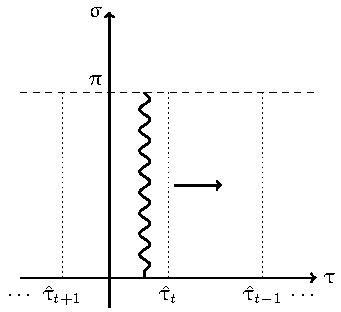
\includegraphics[width=0.4\linewidth]{img/point-like-defects}
  \caption{Propagation of the string in the presence of the worldsheet defects.}
  \label{fig:point-like-defects}
\end{figure}
The boundary conditions are instead:
\begin{equation}
  \eval{
    \qty(
      \var{\psi}_{+,\, i}^* \psi_{+}^{ i} +
      \var{\psi}_{-,\, i}^* \psi_{-}^{ i} -
      \psi_{+,\, i}^* \var{\psi}_{+}^{ i} -
      \psi_{-,\, i}^* \var{\psi}_{-}^{ i}
    )
  }_{\sigma = 0}^{\sigma = \pi} = 0.
  \label{eq:boundary-conditions}
\end{equation}
We solve the constraint imposing the non trivial relations:
\begin{equation}
  \begin{cases}
    \psi_-^i( \tau, 0 )
    =
    \tensor{\qty( R_{(t)} )}{^i_j}
    \psi^j_+( \tau, 0 ),
    & \qquad
    \tau \in \qty( \htau_{(t)}, \htau_{(t-1)} ),
    \\
    \psi_-^i( \tau, \pi )
    =
    - \psi_+^i( \tau, \pi ),
    & \qquad
    \tau \in \R,
  \end{cases}
  \label{eq:boundary-conditions-solutions}
\end{equation}
where $t = 1, 2, \dots, N$.
This way we introduce $N$ zero-dimensional defects on the boundary, pictorially shown in~\Cref{fig:point-like-defects}.
They are located on the strip at $( \htau_{(t)}, 0 ) \in \Sigma$ such that $\htau_{(t)} < \htau_{(t-1)}$ with $\htau_{N+1} = -\infty$ and $\htau_0 = +\infty$.
Their characterisation is given by $N$ matrices $R_{(t)} \in \U{N_f}$.
    
In most of this paper we want the in- and out-vacua to be the usual NS vacuum.
We thus choose the boundary condition at $\sigma = \pi$ so that when there are no defects the system describes NS fermions.
We require also the cancellation of the action of the defects at $\htau = \pm\infty$, that is:
\begin{equation}
  R_{(N)} R_{(N-1)} \dots R_{(1)} = \1.
\end{equation}
More general cases where the asymptotic vacua are twisted can be worked out in similar fashion.
   
In order to connect to the Euclidean formulation we introduce $N_f$ ``double fields'' $\Psi^i$.\footnotemark{}
\footnotetext{%
  In this case they correspond to the fields $\psi^i_+$.
}
They can be obtained by gluing $\psi^i_+$ and $\psi^i_-$ along the $\sigma = \pi$ boundary and labeled by an index $i = 1,\, 2,\, \dots,\, N_f$:
\begin{equation}
  \Psi^i(\tau,\, \phi)
  =
  \begin{cases}
    \psi^i_+(\tau,\, \phi),
    & \qquad 0\le\phi\le \pi
    \\
    -\psi^i_-(\tau,\, 2\pi-\phi),
    & \qquad \pi \le \phi \le 2 \pi        
  \end{cases}
  \label{eq:double-field-Lorentzian}
\end{equation}
where $0 \le \phi \le 2 \pi$.
The boundary conditions become:
\begin{equation}
  \Psi^i(\tau, 2 \pi )
  =
  - \tensor{\qty( R_{(t)} )}{^i_j}
  \Psi^j(\tau,\, 0 ),
  \qquad
  \tau \in \qty( \htau_{(t)},\, \htau_{(t-1)} ).
\end{equation}
Using the equation of motion we get $\Psi^i(\tau,\, \phi) = \Psi^i(\tau + \phi)$ and the boundary conditions become the (pseudo-)periodicity conditions
\begin{equation}
  \Psi^i(\tau + 2 \pi )
  =
  - \tensor{\qty( R_{(t)} )}{^i_j}
  \Psi^j(\tau ),
  \qquad
  \tau \in \qty( \htau_{(t)}, \htau_{(t-1)} ).
\end{equation}
The main issue is now to expand $\Psi$ in a basis of modes and proceed to its quantization.
Even in the simplest case $N_f = 1$ the task of finding the Minkowskian modes turns out to be fairly complicated.
It is however possible to overcome the issue in the Euclidean formalism.


\subsection{Conserved Product and Charges}
\label{sec:product}

In order to promote the theory to its quantum formulation, we define a procedure to build a Fock space of states in the Heisenberg formalism.
Equal time anti-commutation relations must then be invariant in time.
We thus need a time independent internal product to extract the creation and annihilation operators and expand the fields on the basis of modes.


\subsubsection{Conserved Product and Current}

Start from a generic conserved current
\begin{equation}
  j( \tau,\, \sigma )
  =
  j_{\tau}( \tau,\, \sigma )\, \dd{\tau} + j_{\sigma}( \tau,\, \sigma )\, \dd{\sigma},
\end{equation}
and consider
\begin{equation}
  \star j
  =
  j_{\sigma} \dd{\tau} + j_{\tau} \dd{\sigma}
  \quad
  \Rightarrow
  \quad
  \dd{(\star j)}
  =
  \qty( \ipd{\tau} j_{\tau} - \ipd{\sigma} j_{\sigma} ) \dd{\tau} \dd{\sigma},
\end{equation}
where $\star$ is the Hodge dual operator.
Integration over the surface $\Sigma' = [ \tau_i, \tau_f ] \times [ 0, \pi ]$ yields:
\begin{equation}
  \int\limits_{\Sigma'} \dd{(\star j)}
  =
  \int\limits_{\partial \Sigma'}
  \star j
  =
  0
  \qquad
  \Leftrightarrow
  \qquad
  \finiteint{\sigma}{0}{\pi}
  \eval{j_{\tau}}_{\tau = \tau_f}^{\tau = \tau_i}
  =
  \finiteint{\tau}{\tau_i}{\tau_f}
  \eval{j_{\sigma}}_{\sigma = \pi}^{\sigma = 0}.
\end{equation}
The current $j_{\tau}( \tau,\, \sigma )$ is thus conserved in time if
\begin{equation}
  \finiteint{\tau}{\tau_i}{\tau_f}
  \qty( \eval{j_{\sigma}}_{\sigma = \pi} - \eval{j_{\sigma}}_{\sigma = 0} )
  =
  0.
  \label{eq:time-conservation}
\end{equation}
In this case we can define
\begin{equation}
  Q = \finiteint{\sigma}{0}{\pi} j_{\tau}( \tau,\, \sigma ) 
\end{equation}
as conserved quantity (that is $\ipd{\tau} Q = 0$).
We now consider explicitly the symmetries of the action~\eqref{eq:cft-action}.
We focus on diffeomorphism invariance and $\U{N_f}$ flavour symmetries of the bulk theory leading to the stress-energy tensor and a vector current.


\subsubsection{Flavour Vector Current}

Consider first the $\U{N_f}$ vector current of the flavour symmetry in~\eqref{eq:cft-action_full}.
We write it as
\begin{equation}
  j_{\alpha}^a ( \tau,\, \sigma )
  =
  \tensor{\qty( \rT^a )}{^i_j}\,
  \bpsi_i( \tau,\, \sigma )\, \gamma_{\alpha}\, \psi^j( \tau,\, \sigma ),
\end{equation}
where $\rT^a$ is a generator of $\U{N_f}$ such that $a = 1,\, 2,\, \dots,\, N_f^2$.\footnotemark{}
\footnotetext{%
  The results however are more general and hold for a generic matrix $M$ taking the place of any of the generators $\rT^a$.
  Spinors $\psi$ and $\bpsi$ can also be generalized to two different and arbitrary solutions of the \eom~\eqref{eq:eom} while keeping the current conserved.
}
In components we have:
\begin{eqnarray}
  j^a_{\tau}( \tau,\, \sigma )
  & = &
  \tensor{\qty( \rT^a )}{^i_j}\,
  \qty( \psi^*_{+,\, i} \psi^j_+ + \psi^*_{-,\, i} \psi^j_- )
  \\
  j^a_{\sigma}( \tau,\, \sigma )
  & = &
  \tensor{\qty( \rT^a )}{^i_j}\,
  \qty( \psi^*_{+,\, i} \psi^j_+ - \psi^*_{-,\, i} \psi^j_- ).
\end{eqnarray}

In order to define a conserved charge, we require:
\begin{equation}
  \finiteint{\tau}{\tau_i}{\tau_f}
  \qty(
    \eval{j_{\sigma}^a}_{\sigma = \pi} - \eval{j_{\sigma}^a}_{\sigma = 0}
  )
  =
  0,
\end{equation}
where
\begin{equation}
  \eval{j_{\sigma}^a( \tau,\, \sigma )}_{\sigma = \pi} \equiv 0
\end{equation}
using the boundary conditions~\eqref{eq:boundary-conditions}.
Moreover we have:
\begin{equation}
  \eval{j_{\sigma}^a( \tau,\, \sigma )}_{\sigma = 0}
  =
  \qty[
    \psi^*_+\,
    \qty( \rT^a - R_{(t)}^{\dagger} \rT^a R_{(t)} )\,
    \psi_+
  ]_{\sigma = 0},
  \qquad
  \tau \in \qty( \htau_{(t)}, \htau_{(t-1)} ).
\end{equation}
In general
\begin{equation}
  \eval{j_{\sigma}^a( \tau,\, \sigma )}_{\sigma = 0}
  =
  0
  \qquad
  \Leftrightarrow
  \quad
  \rT^a \propto \1
\end{equation}
so that $R_{(t)}^{\dagger} \rT^a = \rT^a R_{(t)}^{\dagger}$.
This shows that the presence of the point-like defects on the worldsheet breaks the $\U{N_f}$ symmetry down to a \U{1} phase.\footnotemark{}
\footnotetext{%
  The symmetry is $\SO{N_f} \times \SO{N_f}$ if we consider Majorana-Weyl fermions.
}
The \U{1} vector current then defines a conserved charge for a restricted class of functions.

Let $\alpha$ and $\beta$ be two arbitrary (bosonic) solutions to the \eom~\eqref{eq:eom}, we define a product
\begin{equation}
  \consprod{\alpha}{\beta}
  =
  \cN
  \finiteint{\sigma}{0}{\pi}
  \qty( \alpha_{+,\, i}^* \beta_+^i + \alpha_{-,\, i}^* \beta_-^i ),
  \label{eq:conserved-product}
\end{equation}
where $\cN \in \R$ is a normalisation constant and the integrand must not present non integrable singularities.
The product is such that $\consprod{\alpha}{\beta} = \consprod{\alpha}{\beta}^*$.
We can also rewrite the result to the double fields defined in~\eqref{eq:double-field-Lorentzian}.
Let in fact $A$ and $B$ be the ``double
fields'' corresponding to $\alpha$ and $\beta$ respectively:
\begin{equation}
  \consprod{\alpha}{\beta}
  =
  \cN
  \finiteint{\phi}{0}{2\pi}\,
  A_i^*( \tau + \phi )\, B^i( \tau + \phi ).
  \label{eq:conserved-product-double-field}
\end{equation}

\subsubsection{Stress-Energy Tensor}

Consider the stress-energy tensor of the bulk theory.
Using the usual Nöther's procedure we get the on-shell non vanishing components:
\begin{equation}
  \begin{split}
    \cT_{++}( \xi_+ )
    & =
    -i \frac{T}{4} \psi_{+,\, i}^*( \xi_+ ) \lrpartial{+} \psi_+^i( \xi_+ ),
    \\
    \cT_{--}( \xi_- )
    & =
    -i \frac{T}{4} \psi_{-,\, i}^*( \xi_- )\lrpartial{-} \psi_-^i( \xi_- ).
  \end{split}
  \label{eq:stress-energy-tensor-lightcone}
\end{equation}
As always the boundary of $\Sigma$ breaks the symmetry for translations in the $\sigma$ direction, while the defects break the time translations: the Hamiltonian is therefore time-dependent but it is constant between two consecutive point-like defects.
In fact, from the definition of the stress-energy tensor, we can in principle
build the hypothetical charges:
\begin{eqnarray}
  \rH( \tau )
  & = &
  \finiteint{\sigma}{0}{\pi}
  \cT_{\tau\tau}( \tau,\, \sigma )
  =
  \finiteint{\sigma}{0}{\pi}
  \qty( \cT_{++}( \tau + \sigma ) + \cT_{--}( \tau - \sigma ) ),
  \label{eq:hamiltonian}
  \\
  \rP( \tau )
  & = &
  \finiteint{\sigma}{0}{\pi}
  \cT_{\tau\sigma}( \tau,\, \sigma )
  =
  \finiteint{\sigma}{0}{\pi}
  \qty( \cT_{++}( \tau + \sigma ) - \cT_{--}( \tau - \sigma ) ),
  \label{eq:momentum}
\end{eqnarray}
which are conserved if~\eqref{eq:time-conservation} holds.

We order the point-like defects as $\htau_{(t_0 - 1)} < \tau_i \le \htau_{(t_0)} < \htau_{(t_N)} \le \tau_f < \htau_{(t_N+1)}$.
For the linear momentum $\rP$ the condition of conservation
reads:\footnotemark{}
\footnotetext{%
  Notice that in the second term of the second line the differentiation with respect to $\tau$ is acting only on $R_{(t)}$ and $R_{(t)}^{\dagger}$.
}
\begin{equation}
  \begin{split}
    & \finiteint{\tau}{\tau_i}{\tau_f}
    \eval{\qty( \cT_{++}( \tau + \sigma ) + \cT_{--}( \tau - \sigma ) )}_{\sigma = 0}^{\sigma = \pi}
    \\
    & =
    - i \frac{T}{4}
    \int \Delta\tau
    \qty(
      2 \eval{\psi_{+,\, i}^*\, \lrpartial{\tau} \psi_+^i}^{\sigma = \pi}_{\sigma = 0}
      -
      \eval{\psi_{+,\, i}^* \tensor{\qty( R_{(t)}^{\dagger} \lrpartial{\tau} R_{(t)} )}{^i_j} \psi_+^j}_{\sigma = 0}
    )
    \neq
    0.
  \end{split}
\end{equation}
The corresponding condition for the Hamiltonian $\rH$ is:
\begin{equation}
  \begin{split}
    & \finiteint{\tau}{\tau_i}{\tau_f}
    \eval{\qty( \cT_{++}( \tau + \sigma ) - \cT_{--}( \tau - \sigma ) )}_{\sigma = 0}^{\sigma = \pi}
    \\
    & =
    - i \frac{T}{4}
    \int \Delta\tau
    \qty( \eval{\psi_{+,\, i}^* \tensor{\qty( R_{(t)}^{\dagger} \lrpartial{\tau} R_{(t)} )}{^i_j} \psi_+^j}_{\sigma = 0} )
    = 0
    \quad
    \Leftrightarrow
    \quad
    \qty( \tau_i, \tau_f ) \in \qty( \htau_{(t)}, \htau_{(t-1)} ).
  \end{split}
\end{equation}
In both cases we used the shorthand graphical notation
\begin{equation}
    \int \Delta \tau
    =
    \qty(
      \int\limits_{\tau_i}^{\htau_{t_0}}
      +
      \finitesum{t}{t_0}{t_N - 1}
      \int\limits_{\htau_{(t)}}^{\htau_{(t+1)}}
      +
      \int\limits_{\htau_N}^{\tau_f}
    )
    \dd{\tau}
\end{equation}
for simplicity.

These relations therefore prove that the generator of the $\sigma$-translations~\eqref{eq:momentum} is not conserved in time because of the boundary conditions, while the time evolution operator $\rH$ is only piecewise conserved and therefore globally time dependent.


\subsection{Basis of Solutions and Dual Modes}

Let $\qty{ \psi_{n,\, \pm}^i }_{n \in \Z}$ be a complete basis of modes such that:
\begin{equation}
  \begin{cases}
    \psi_{n,\, +}^i( \tau, 0 ) = \qty( R_{(t)} )^i_j \psi_{n,\, -}^j(
    \tau, 0 ) & \qfor \tau \in \qty( \htau_{(t)}, \htau_{(t-1)} )
    \\
    \psi_{n,\, +}^i( \tau, \pi ) = -\psi_{n,\, -}^i( \tau, \pi )
    & \qfor \tau \in \R
  \end{cases}.
\end{equation}
These fields are related to a complete basis of the modes of the ``double field'' $\Psi_n^i$ as in~\eqref{eq:double-field-Lorentzian}.
The modes $\psi_n$ (and their counterparts $\Psi_n$) are a basis of solutions of the \eom and the boundary conditions for $\tau \in \R \setminus \qty{ \htau_{(t)} }_{0 \le t \le N}$.
The fields $\psi^i$ (and the fields $\Psi^i$) are then a superposition of such modes:
\begin{equation}
  \psi^i_{\pm}( \xi_{\pm} )
  =
  \sum\limits_{n \in \Z} b_n\, \psi^i_{n,\, \pm}( \xi_{\pm} )
  \qquad
  \Rightarrow
  \qquad
  \Psi^i( \xi )
  =
  \sum\limits_{n \in \Z} b_n\, \Psi^i_n( \xi ).
\label{eq:usual-mode-expansion}
\end{equation}

In order to extract the ``coefficients'' $b_n$ we first introduce the dual basis $\dual{\psi}_{n,\, \pm}$ (and $\dual{\Psi}_n$) in an abstract sense such that:
\begin{itemize}
  \item the dual fields $\dual{\psi}_{n,\, \pm}$ (and $\dual{\Psi}_n$) must be solutions to the \eom,

  \item the dual fields $\dual{\psi}_{n,\, \pm}$ (and $\dual{\Psi}_n$) can differ from $\psi_{n,\, \pm}$ (and $\Psi_n$) in their behavior at the boundary,

  \item the functional form of $\dual{\psi}_{n,\, \pm}$ (and $\dual{\Psi}_n$) is fixed by the request of time invariance of the usual anti-commutation relations $\qty[ b_n, b_m^{\dagger} ]_+$ (that is $b_n$ and $b_n^{\dagger}$ can evolve in time, but their anti-commutation relations must remain constant).
\end{itemize}
We then define the conserved product for the ``double fields''~\eqref{eq:conserved-product-double-field} in such a way that:
\begin{equation}
  \eval{\lconsprod{\dual{\Psi}_n}{\Psi_m}}_{\tau = \tau_0}
  =
  \cN
  \finiteint{\sigma}{0}{2\pi}
  \dual{\Psi}_{n,\, i}^{*}(\tau + \sigma)\,
  \Psi_m^i( \tau + \sigma )
  =
  \delta_{n,\, m}.
  \label{eq:conserved-product-dual-basis}
\end{equation}
In the previous expression we changed the notation of the product.
We are in fact dealing with the space of solutions whose basis is $\qty{ \Psi_n }$ and a dual space with basis $\qty{ \dual{\Psi}_n }$ which is not required to span entirely the original space but only to be a subset of it in order to be able to compute the anti-commutation relations among the annihilation and construction operators in a well defined way as in~\eqref{eq:Mink_can_anticomm_rel_ann_des}.
Given the previous product we can extract the operators as
\begin{eqnarray}
  \lconsprod{\dual{\Psi}_n}{\Psi} & = & b_n,
  \\
  \lconsprod{\dual{\Psi}_n^*}{\Psi^*} & = & b_n^{\dagger}.
\end{eqnarray}
As a consequence of the canonical anti-commutation relations
\begin{equation}
  \qty[
    \Psi^i\qty( \tau,\, \sigma ), \Psi^*_j\qty( \tau,\, \sigma' )
  ]_+
  =
  \frac{2}{T}\, \tensor{\delta}{^i_j}\, \delta( \sigma - \sigma' ),
\end{equation}
we have then:
\begin{equation}
  \eval{\qty[ b_n, b_m^{\dagger} ]_+}_{\tau = \tau_0}
  =
  \frac{2}{T} \cN \eval{\lconsprod{\dual{\Psi}_n}{\dual{\Psi}_m}}_{\tau = \tau_0}.
  \label{eq:Mink_can_anticomm_rel_ann_des}
\end{equation}
By definition the product~\eqref{eq:conserved-product-dual-basis} is time independent as long as the integrand $\dual{\Psi}_n^* \Psi_m$ is free of singularities at $\tau = \htau_{(t)}$ for $t = 1, 2, \dots, N$.
Such request on the dual basis automatically fixes its functional form.
Clearly this does not exclude the possibility to have singularities in $\Psi_m$ or $\dual{\Psi}_n$ separately: they are instead deeply connected to the boundary changing primary operator hidden in the discontinuity of the boundary conditions, that is different singularities will be shown to be in correspondence to the excited spin fields.
Using the definition of the conserved product we therefore moved the focus from finding a consistent definition of the Fock space to the construction of the dual basis of modes.
This task is however easier to address in a Euclidean formulation.


\subsection{Point-like Defect CFT: the Euclidean Formulation}
\label{sec:eucl_formulation}

In the Euclidean reformulation the solution to the \eom might be easier to study than its Lorentzian worldsheet form.
This is specifically the case when $R_{(t)} \in \U{1}^{N_f} \subset \U{N_f}$.
The presence of a time dependent Hamiltonian is not standard and we can neither blindly apply the usual Wick rotation nor the usual CFT techniques.


\subsubsection{Fields on the Strip}

Performing the Wick rotation as $\tau_E = i \tau$ such that $e^{i S} = e^{-S_E}$, the Minkowskian action~\eqref{eq:cft-action} becomes:
\begin{equation}
  S_E
  =
  \frac{T}{2}
  \iint \dd{\xi} \dd{\bxi}\,
  \frac{1}{2}\,
  \qty(
    \hpsi_{E,\, +,\, i}^*\, \lrpartial{\bxi} \hpsi_{E,\, +}^i
    +
    \hpsi_{E,\, -,\, i}^*\, \lrpartial{\xi} \hpsi_{E,\, -}^i
  ),
  \label{eq:S_Eu_strip}
\end{equation}
where the Euclidean fermion on the strip is connected to the Minkowskian formulation through
\begin{equation}
  \hpsi_{E,\, \pm}^i( \xi,\, \bxi )
  =
  \psi_{\pm}^i( -i\xi,\, -i\bxi ).
\end{equation}
In the previous expressions we defined the coordinates $\xi = \tau_E + i \sigma$, $\bar \xi = \tau_E - i \sigma$ such that $\bxi = \xi^*$.
Moreover we get $\ipd{\xi} = \pdv{\xi} = \frac{1}{2} \qty( \pdv{\tau_E} - i\pdv{\sigma} )$, $\ipd{\bxi} = \pdv{\bxi} = \frac{1}{2} \qty( \pdv{\tau_E} + i \pdv{\sigma} )$.
As a consequence the Euclidean ``complex conjugation'' $\star$ (defined off-shell) acts as
\begin{equation}
  \qty[
    \hpsi_{E,\, \pm}^i(\xi,\, \bxi)
  ]^\star
  =
  \hpsi_{E,\, \pm i}^*(-\bxi,\, -\xi).
  \label{eq:off-shell-Hermitian-conjugate}
\end{equation}

The \eom are as usual
\begin{eqnarray}
  \ipd{\xi} \hpsi_{E,\, -}^i( \xi,\, \bxi )
  = &
  \ipd{\bxi} \hpsi_{E,\, +}^i( \xi,\, \bxi )
  = &
  0,
  \\
  \ipd{\xi} \hpsi_{E,\, -,\, i}^*( \xi,\, \bxi )
  = &
  \ipd{\bxi} \hpsi_{E,\, +,\, i}^*( \xi,\, \bxi )
  = &
  0,
\end{eqnarray}
whose solutions are the holomorphic functions $\hpsi_{E,\, +}( \xi )$ and $\hpsi_{E,\, -}( \bxi )$, together with $\hpsi_{E,\, +}^*( \xi )$ and $\hpsi_{E,\, -}^*( \bxi )$.
In these coordinates the boundary conditions~\eqref{eq:boundary-conditions-solutions} translate to:
\begin{equation}
  \begin{cases}
    \hpsi_{E,\, -}^i( \tau_E - i\, 0^+ )
    & =
    \tensor{\qty( R_{(t)} )}{^i_j}\,
    \hpsi_{E,\, +}^j(\tau_E + i\, 0^+ )
    \\
    \hpsi_{E,\, -,\, i}^{*}( \tau_E - i\, 0^+ )
    & =
    \tensor{\qty( R_{(t)}^* )}{_i^j}\,
    \hpsi_{E,\, +,\, j}^*(\tau_E + i\, 0^+ )
  \end{cases}
  \label{eq:bc_eu_strip}
\end{equation}
for $\tau_E \in \qty( \htau_{E,\, (t)}, \htau_{E,\, (t-1)} )$ and
\begin{equation}
  \begin{cases}
    \hpsi_{E,\, -}^i( \tau_E - i\, \pi )
    & =
    -\hpsi_{E,\, +}^i( \tau_E + i\, \pi )
    \\
    \hpsi_{E,\, -,\, i}^*( \tau_E - i\, \pi )
    & =
    -\hpsi_{E,\, +,\, i}^*( \tau_E + i\, \pi )
  \end{cases},
\end{equation}
where $t = 1,\, 2,\, \dots,\, N$ and $\htau_{E,\, (t)}$ are the Wick-rotated locations of the $N$ zero-dimensional defects, analytically continued to a real value.

The conserved product on the strip becomes:
\begin{equation}
  \consprod{\halpha^*_E}{\hbeta_E}
  =
  \cN
  \finiteint{\sigma}{0}{\pi}
  \qty(
    \halpha^*_{E,\, +,\, i} \hbeta_{E,\, +}^i
    +
    \halpha^*_{E,\, -,\, i}  \hbeta_{E,\, -}^i
  ),
  \label{eq:euclidean-conserved-product-strip}
\end{equation}
where $\halpha^*_E$ and $\hbeta_E$ are the Euclidean counterparts of the generic solutions in the original definition of the product in~\eqref{eq:conserved-product}.
In the Euclidean context we have to explicitly write $\halpha^*_E$ because it is no longer the ``complex conjugate''  of $\halpha_E$ in the traditional sense.
The product is conserved only when it couples two solutions which have different boundary conditions as in~\eqref{eq:bc_eu_strip}.

The definition of the stress-energy tensor in~\eqref{eq:stress-energy-tensor-lightcone} requires a change in the numerical pre-factor to use the usual CFT normalization.
Introducing a spacetime variable central charge as well the components of the stress-energy tensor become:\footnotemark{}
\footnotetext{%
  The canonical coefficient in front of the CFT stress-energy tensor is such that the Euclidean Hamiltonian $\rL_{0}$ is normalized such that
  \begin{equation*}
    \cT_{\zeta\zeta}( \zeta ) = \sum_n \rL_{n} e^{-n \zeta}
  \end{equation*}
  (we are anticipating the double strip notation defined in the next subsection for simplicity).
  We thus get:
  \begin{equation*}
     \rH_E
     =
     \rL_{0}
     =
     \int\limits_{0}^{2\pi} \frac{\dd{\phi}}{2 \pi}
     \cT_{\zeta \zeta}( \tau_E + i\, \phi )
  \end{equation*}
  therefore $\cT_{\zeta\zeta}( \zeta ) = 2 \pi\, \cT^{(can)}_{\zeta\zeta}( \zeta )$.
}
\begin{equation}
  \begin{split}
    \cT_{\xi \xi}( \xi )
    & =
    - \frac{\pi T}{2}\,
    \hpsi_{E,\, +,\, i}^*( \xi )\, \lrpartial{\xi} \hpsi^i_{E,\, +}( \xi )
    +
    \widehat{\cC}( \xi ),
    \\
    \cT_{\bxi \bxi}( \bxi )
    & =
    - \frac{\pi T}{2}\,
    \hpsi_{E,\, -,\, i}^*( \bxi ) \lrpartial{\bxi}
    \hpsi^i_{E,\, -}( \bxi )
    +
    \widehat{\overline{\cC}}( \bxi ),
  \end{split}
\end{equation}
where $\widehat{\cC}$ and $\widehat{\overline{\cC}}$ are the leftover terms after the regularization of the singularities due to the normal ordering.
The canonical anti-commutation relations are then
\begin{equation}
  \eval{
    \qty[
      \hpsi_{E,\, \pm}^i( \xi_1,\, \bxi_1),
      \hpsi_{E,\, \pm,\, j}^*( \xi_2,\, \bxi_2 )
    ]_+
  }_{\Re\xi_1 = \Re\xi_2}
  =
  \frac{2}{T}\,
  \tensor{\delta}{^i_j}\,
  \delta\qty( \Im\xi_1 - \Im\xi_2 ).
\end{equation}

Given the Euclidean modes $\hpsi^i_{E,\, \pm,\, n}$ and $\hpsi^*_{E,\, \pm,\, n,\, i}$ where $n \in \Z$, we can then define the dual modes $\dual{\hpsi}^i_{E,\, n}$ and $\dual{\hpsi}^*_{E,\, n,\, i}$ such that the conserved product~\eqref{eq:euclidean-conserved-product-strip} between them gives:
\begin{equation}
  \lconsprod{\dual{\hpsi}^*_{E,\, n}}{\hpsi_{E,\, m}}
  =
  \lconsprod{\dual{\hpsi}_{E,\, n}}{\hpsi^*_{E,\, m}}
  =
  \delta_{n,m}.
\end{equation}
We can then expand the fields as
\begin{equation}
  \begin{cases}
    \hpsi^i_{E,\, +}(\xi)
    & =
    \sum\limits_{n \in \Z} b_n\, \hpsi^i_{E,\, +,\, n}(\xi)
    \\
    \hpsi^i_{E,\, -}(\bxi)
    & =
    \sum\limits_{n \in \Z} b_n\, \hpsi^i_{E,\, -,\, n}(\bxi)
  \end{cases}
\end{equation}
and
\begin{equation}
  \begin{cases}
    \hpsi^*_{E,\, +,\, i}(\xi)
    & =
    \sum\limits_{n \in \Z} b^*_n\, \hpsi^*_{E,\, +,\, n,\, i}(\xi)
    \\
    \hpsi^*_{E,\, -,\, i}(\bxi)
    & =
    \sum\limits_{n \in \Z} b^*_n\, \hpsi^*_{E,\, -,\, n,\, i}(\bxi)
  \end{cases}
\end{equation}
in order to extract the operators through the conserved product
\begin{equation}
  b_n
  =
  \lconsprod{\dual{\hpsi}^*_{E,\, n}}{\hpsi_{E}},
  \qquad
  b^*_n
  =
  \lconsprod{\dual{\hpsi}_{E,\, n}}{\hpsi^*_{E}},
\end{equation}
and get the anti-commutation relations at fixed Euclidean time as
\begin{equation}
  \eval{ \qty[ b_n,\, b^*_m ]_+ }_{\tau_E = \tau_{E,\, (0)}}
  =
  \frac{2 \cN}{T}
  \lconsprod{\dual{\hpsi}^*_{E,\, n}}{\dual{\hpsi}_{E,\, m}}.
\end{equation}


\subsubsection{Double Strip Formalism and Doubling Trick}

It is natural to use the doubling trick on the strip to simplify the previous expressions by gluing the holomorphic and anti-holomorphic fields along the $\sigma = \pi$ boundary.
Define the coordinate $\zeta = \tau_E + i\, \phi$ with $0 \le \phi \le 2\pi$.
We then have
\begin{equation}
  \Hpsi( \zeta )
  =
  \begin{cases}
    \hpsi_{E,\, +}(\zeta)
    &
    \qfor
    \phi = \sigma \in \qty[ 0, \pi ]
    \\
    -\hpsi_{E,\, -}(\zeta - 2 \pi i)
    &
    \qfor
    \phi = 2\pi - \sigma \in \qty[ \pi, 2 \pi ]
  \end{cases}
\end{equation}
on-shell (and similarly for $\Hpsi^*( \zeta )$ with the substitution $\hpsi_{E,\, \pm} \to \hpsi_{E,\, \pm}^*$).
The ``complex conjugation'' $\star$ acts on the off-shell double fields as
\begin{equation}
  \qty[ \Hpsi^i(\zeta,\, \bzeta) ]^\star = \Hpsi_i^*(-\bzeta,\, -\zeta),
\end{equation}
while the boundary conditions are translated into
\begin{equation}
  \begin{cases}
    \Hpsi^i( \tau_E + 2 \pi i^- )
    =
    -\tensor{\qty( R_{(t)} )}{^i_j}\,
    \Hpsi^j( \tau_E + i\, 0^+ )
    \\
    \Hpsi^{* i}( \tau_E + 2 \pi i^- )
    =
    -\tensor{\qty( R_{(t)}^* )}{^i_j}\,
    \Hpsi^{* j}( \tau_E + i\, 0^+ )
  \end{cases}
\end{equation}
for $\tau_E \in \qty( \htau_{E,\, (t)}, \htau_{E,\, (t-1)} )$.
The conserved product can then be defined as
\begin{equation}
  \consprod{\widehat{A}^*}{\widehat{B}}
  =
  \cN
  \finiteint{\phi}{0}{2\pi}\,
  \widehat{A}^*_i(\tau_E + i\, \phi )\,
  \widehat{B}^i( \tau_E + i\, \phi ),
\end{equation}
where $\widehat{A}^*$ and $\widehat{B}$ are the double fields connected to $\halpha^*_E$ and $\hbeta_E$ in the previous definition on the strip.
The holomorphic stress-energy tensor is then
\begin{equation}
  \cT_{\zeta \zeta}( \zeta )
  =
  - \frac{\pi T}{2}\,
  \Hpsi_{i}^*( \zeta )\, \lrpartial{\zeta} \Hpsi^i( \zeta ) 
  +
  \widehat{\cC}(\zeta)
\end{equation}
and the canonical anti-commutation relations are now
\begin{equation}
  \eval{
    \qty[
      \Hpsi^i( \zeta_1 )
      ,
      \Hpsi_{j}^*( \zeta_2 )
    ]_+
  }_{\Re\zeta_1 = \Re\zeta_2}
  =
  \frac{2}{T}\, \tensor{\delta}{^i_j} \delta\qty( \Im\zeta_1 - \Im\zeta_2 ).
\end{equation}


The double field formulation shows that we need only one coefficient $b_n$ (or $b_n^*$) for both $\psi_{E,\, +}$ and $\psi_{E,\, -}$ (or for both $\psi^*_{E,\, +}$ and $\psi^*_{E,\, -}$).
In fact, given the Euclidean modes $\Hpsi^i_{n}$ and $\Hpsi^*_{n,\, i}$ where $n \in \Z$, we define the dual modes $\dual{\Hpsi}^i_{n}$ and $\dual{\Hpsi}^*_{n,\, i}$ such that:
\begin{equation}
  \lconsprod{\dual{\Hpsi}^*_{n}}{\Hpsi_{m}}
  =
  \lconsprod{\dual{\Hpsi}_{n}}{\Hpsi^*_{m}}
  =
  \delta_{n,m}.
\end{equation}
We expand the double fields as
\begin{equation}
  \Hpsi^i(\zeta)
  =
  \sum\limits_{n \in \Z} b_n \Hpsi^i_{n}(\zeta),
  \qquad
  \Hpsi^*_{i}(\zeta)
  =
  \sum\limits_{n \in \Z} b^*_n \Hpsi^*_{n}(\zeta)
\end{equation}
Operators are then extracted as
\begin{equation}
  b_n
  =
  \lconsprod{\dual{\Hpsi}^*_{n}}{\Hpsi},
  \qquad
  b^*_n
  =
  \lconsprod{\dual{\Hpsi}_{n}}{\Hpsi^*}.
  \label{eq:upper-half-extraction}
\end{equation}
Finally we get the anti-commutation relations as
\begin{equation}
  \eval{ \qty[ b_n, b^*_m ]_+ }_{\tau_E = \tau_{E,\, 0}}
  =
  \frac{2 \cN}{T} \lconsprod{\dual{\Hpsi}^*_{n}}{\dual{\Hpsi}_m}.
\end{equation}


\subsection{Fields on the Upper Half Plane}

\begin{figure}[tbp]
  \centering
  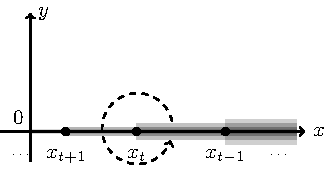
\includegraphics[width=0.5\linewidth]{img/complex-plane}
  \caption{%
    Fields are glued on the $x < 0$ semi-axis with non trivial discontinuities for $x_t < x < x_{t-1}$ for $t = 1,\, 2,\, \dots,\, N$ and where $x_t = \exp( \htau_{E,\, (t)} )$.
  }
  \label{fig:complex-plane}
\end{figure}

We consider a set of coordinates on the upper half \ccH of the complex plane:
\begin{equation}
  u = e^{\xi} \in \ccH,
\end{equation}
where $\xi = \tau_E + i \sigma$ and $\sigma \in \qty[ 0, \pi ]$ define the usual strip, and $\ccH = \qty{ w \in \C \mid \Im w \ge 0 }$.
These coordinates can then be extended to the entire complex plane by considering
\begin{equation}
  z = e^{\zeta} \in \C,
\end{equation}
where $\zeta = \tau_E + i \phi$ and $\phi \in \qty[0, 2\pi ]$ define the double strip.
Under this change of coordinates the Euclidean action~\eqref{eq:S_Eu_strip} becomes
\begin{equation}
  \begin{split}
    S_E
    & =
    \frac{T}{2}
    \iint \dd{u}\dd{\bu}\,
    \frac{1}{2}\,
    \qty(
      \frac{1}{u}\, \hpsi_{E,\, +,\, i}^* \lrpartial{\bu} \hpsi_{E,\, +}^i
      +
      \frac{1}{\bu}\, \hpsi_{E,\, -,\, i}^* \lrpartial{u} \hpsi_{E,\, -}^i
    )
    \\
    & =
    \frac{T}{2}
    \iint \dd{u}\dd{\bu}\,
    \frac{1}{2}\,
    \qty(
      \psi_{E,\, +,\, i}^* \lrpartial{\bu} \psi_{E,\, +}^i
      +
      \psi_{E,\, -,\, i}^* \lrpartial{u} \psi_{E,\, -}^i
    ),
  \end{split}
\end{equation}
where we introduce the off-shell field redefinitions:
\begin{equation}
  \psi_{E,\, +}^i(u,\, \bu)
  =
  \frac{1}{\sqrt{u}}\, \hpsi_{E,\, +}^i( \xi,\, \bxi ),
  \qquad
  \psi_{E,\, -}^i(u,\, \bu)
  =
  \frac{1}{\sqrt{\bu}}\, \hpsi_{E,\, -}^i( \xi,\, \bxi ).
  \label{eq:euclidean-off-shell-redefinitions}
\end{equation}
Fields with the hat sign on top thus represent strip and double strip definitions, while fields without the hat sign are defined on $\ccH$ or $\C$.\footnotemark{}
\footnotetext{%
  We could have anticipated these redefinitions from a CFT argument where
    \begin{equation*}
      \psi( u ) = \eval{\qty( \dv{u}{\xi} )^{-\frac{1}{2}}
        {\hpsi}(\xi)}_{\xi = \ln( u )},
    \end{equation*}
  but we cannot and do not rely on CFT properties since we have not shown that the theory is a CFT yet.
}
Notice that this is the result one would expect from the engineering dimension: in this case it works since the theory is essentially free.
Using the redefinitions~\eqref{eq:euclidean-off-shell-redefinitions}, the off-shell ``complex conjugation'' $\star$ then becomes
\begin{equation}
  \qty[ \psi_{E,\, +,\, i}( u,\, \bu ) ]^\star
  =
  \frac{1}{\bu}\, \psi_{E,\, +,\, i}^*\qty( \frac{1}{\bu},\, \frac{1}{u} ),
  \qquad
  \qty[ \psi_{E,\, -,\, i}( u,\, \bu ) ]^\star
  =
  \frac{1}{u}\, \psi_{E,\, -,\, i}^*\qty( \frac{1}{\bu},\, \frac{1}{u} ).
\end{equation}

We choose to insert the cut of the square root on the real negative axis.
The boundary conditions are then translated into
\begin{equation}
  \begin{cases}
    \psi_{E,\, -}^i( x - i\, 0^+ )
    =
    \tensor{\qty( R_{(t)} )}{^i_j} \psi_{E,\, +}^j( x + i\, 0^+ )
    \\
    \psi^{*}_{E,\, -,\, i}( x - i\, 0^+ ) =
    \tensor{\qty( R_{(t)}^* )}{_i^j} \psi^{*}_{E,\, +,\, j}( x + i\, 0^+ )
  \end{cases}
\end{equation}
for $x \in \qty( x_{(t)}, x_{(t-1)} )$, where $x_{(t)} = \exp( \htau_{E,\, (t)} ) > 0$, and
\begin{equation}
  \psi_{E,\, -}^i( x - i\, 0^+ )
  =
  \psi_{E,\, +}^i( x + i\, 0^+ ),
  \qquad
  \psi^{*}_{E,\, -,\, i}( x - i\, 0^+ )
  =
  \psi^{*}_{E,\, +,\, i}( x + i\, 0^+ )
\end{equation}
for $x<0$.

The product~\eqref{eq:euclidean-conserved-product-strip} is then
\begin{equation}
  \consprod{\alpha^*}{\beta}
  =
  -i \cN\,
  \qty[
    \int\limits_{\widehat{\Sigma}} \dd{u}
    \alpha^*_{+,\, i}(u) \beta_+^i(u)
    -
    \int\limits_{\widehat{\overline{\Sigma}}} \dd{\bu}
    \alpha^*_{-,\, i}(\bu) \beta_-^i(\bu)
  ],
  \label{eq:prod_H}
\end{equation}
where integrations are computed over two semi-circles $\widehat{\Sigma} = \qty{ u \in \C \mid \abs{u} = \exp( \htau_E ),\, 0 \le \Im u \le \pi }$ and $\widehat{\overline{\Sigma}} = \qty{ u \in \C \mid \abs{u} = \exp( \htau_E ),\, -\pi \le \Im u \le 0}$.
The stress-energy tensor becomes:\footnotemark{}
\footnotetext{%
  While rewriting the operator part of the stress-energy tensor from the strip
  formulation into the coordinates in $\ccH$ we actually get
  \begin{equation*}
    \cT_{\xi \xi}( \xi(u) ) = u^2\, \cT_{u u}( u ).
  \end{equation*}
  The reason of the presence of $u^2$ factor can be explained in two ways.
  Using GR we know that $\cT_{\xi \xi}( \xi ) \dss[2]{\xi} = \cT_{u u}( u ) \dss[2]{u}$.
  Another way is to notice that a translation in $\xi$ is a dilatation of $u$: the infinitesimal generator of $\xi$ translation must be the infinitesimal
  generator of $u$ dilatation, that is:
  \begin{equation*}
    P_{\xi}
    \sim
    \int \dd{\sigma}\, \cT_{\xi \xi}
    \sim
    D_u
    \sim 
    \int \dd{u}\, u\, \cT_{u u}.
  \end{equation*}
}
\begin{equation}
  \begin{split}
    \cT_{u u}( u )
    & =
    - \frac{\pi T}{2}\,
    \psi_{E,\, +,\, i}^*( u )\, \lrpartial{u} \psi^i_{E,\, +}( u )
    +
    \widehat{\cC}(u ),
    \\
    \cT_{\bu \bu}( \bu )
    & =
    - \frac{\pi T}{2}\,
    \psi_{E,\, -,\, i}^*( \bu )\, \lrpartial{\bu} \psi^i_{E,\, -}( \bu )
    +
    \widehat{\overline{\cC}}( \bu ).
  \end{split}
\end{equation}
Finally the anti-commutation relations are
\begin{equation}
  \begin{cases}
    \eval{
      \qty[
        \psi_{E,\, +}^i( u_1,\, \bu_1 )
        ,
        \psi_{E,\, +,\, j}^*( u_2,\, \bu_2 )
      ]_+
    }_{\abs{u_1} = \abs{u_2}}
    & =
    \frac{2}{T u_1}\, \tensor{\delta}{^i_j}\, \delta( \arg(u_1) - \arg(u_2) )
    \\
    \eval{
      \qty[
        \psi_{E,\, -}^i( u_1,\, \bu_1 )
        ,
        \psi_{E,\, -,\, j}^*( u_2,\, \bu_2 )
      ]_+
    }_{\abs{u_1} = \abs{u_2}}
    & =
    \frac{2}{T \bu_1}\, \tensor{\delta}{^i_j}\, \delta( \arg(u_1) - \arg(u_2) ),
  \end{cases}
\end{equation}
which despite the strange look of the expression are perfectly compatible with the definition~\eqref{eq:upper-half-extraction} leading to:
\begin{equation}
  \qty[ b_n,\, b^*_m ]_+
  =
  \frac{2 \cN}{T}\,
  \lconsprod{\dual{\hpsi}^*_{E,\, n}}{\dual{\hpsi}_{E,\, m}}
  =
  \frac{2 \cN}{T}\,
  \lconsprod{\dual{\psi}^*_{E,\, n}}{\dual{\psi}_{E,\, m}}
\end{equation}
when the product $\lconsprod{\cdot}{\cdot}$ is defined according to~\eqref{eq:prod_H}.
We expand the fields in modes as:
\begin{equation}
  \begin{cases}
    \psi^i_{E,\, +}(u)
    =
    \sum\limits_{n \in \Z} b_n\, \psi^i_{E,\, +,\, n}(u)
    \\
    \psi^i_{E,\, -}(\bu)
    =
    \sum\limits_{n \in \Z} b_n\, \psi^i_{E,\, -,\, n}(\bu)
  \end{cases}
\end{equation}
and
\begin{equation}
  \begin{cases}
    \psi^*_{E,\, +,\, i}(u)
    =
    \sum\limits_{n \in \Z} b^*_n\, \psi^*_{E,\, +,\, n,\, i}(u)
    \\
    \psi^*_{E,\, -,\, i}(\bu)
    =
    \sum\limits_{n \in \Z} b^*_n\, \psi^*_{E,\, -,\, n,\, i}(\bu)
  \end{cases}
\end{equation}
and $\dual{\psi}_{E,\, n}$ and $\dual{\psi}^*_{E,\, n}$ are the corresponding dual modes on the upper half plane.   


\subsection{Fields on the Complex Plane and the Doubling Trick}
  
We use again the doubling trick to define the fields on the subset $\C \setminus \qty[ x_{(N)},\, x_{(1)} ]$:
\begin{equation}
  \Psi( z )
  =
  \begin{cases}
    \psi_{E,\, +}(u)
    & \qfor
    z = u \in \ccH \setminus \qty[ x_{(N)}, x_{(1)} ]
    \\
    \psi_{E,\, -}(\bu)
    & \qfor
    z = \bu \in \overline{\ccH} \setminus \qty[ x_{(N)}, x_{(1)} ]
  \end{cases}
\end{equation}
where $z = \exp( \tau_E + i\, \phi ) = x + i y$ and $\overline{\ccH} = \qty{ w \in \C \mid \Im w \le 0 }$.
The same procedure applies also to $\Psi^*$ with the exchange $\psi_{E,\, \pm} \leftrightarrow \psi_{E,\, \pm}^*$.

In this case the ``complex conjugation'' $\star$ acts off-shell as
\begin{equation}
  \qty[ \Psi^i( z, \bz ) ]^\star
  =
  \frac{1}{\bz}\, \Psi_i^*\qty(\frac{1}{\bz}, \frac{1}{z}).
  \label{eq:complex-plane-conjugate}
\end{equation}
The boundary conditions then become:
\begin{equation}
  \begin{cases}
    \Psi^i( x - i\, 0^+ )
    & =
    \tensor{\qty( R_{(t)} )}{^i_j} \Psi^j( x + i\, 0^+ ),
    \\
    \Psi^{*\, i}( x - i 0^+ )
    & =
    \tensor{\qty( R_{(t)}^* )}{^i_j} \Psi^{*\, j}( x + i\, 0^+ ),
  \end{cases}
  \label{eq:boundary-condition-euclidean}
\end{equation}
for $x \in \qty( x_{(t)}, x_{(t-1)} )$, where $x_{(t)} = \exp( \htau_{E,\, (t)} ) > 0$ for $t \in \qty{ 1,\, 2,\, \dots,\, N }$.
When $x < 0$ we get
\begin{equation}
  \begin{cases}
    \Psi( x - i\, 0^+ ) & = \Psi( x + i\, 0^+ ),
    \\
    \Psi^*( x - i\, 0^+ ) & = \Psi^*( x + i\, 0^+ )
  \end{cases}.
  \label{eq:gluing-conditions-euclidean}
\end{equation}

Given the relations $\dd{z} = i\, z\, \dd{\phi}$, we can write the conserved product \eqref{eq:prod_H} as:
\begin{equation}
  \consprod{A^*}{B}
  =
  2\pi \cN
  \oint\limits_{\abs{z} = \exp( \tau_E )}
  \frac{\dd{z}}{2 \pi i}\, A^*_i( z )\, B^i( z ),
  \label{eq:conserved-product-complex-plane}
\end{equation}
where we explicitly stressed that the integral has to be performed at a fixed Euclidean time $\tau_E$: in the new coordinate on the plane the conserved product becomes a contour integral at a fixed radius from the origin.

In the same way we can recast the stress-energy tensor components~\eqref{eq:stress-energy-tensor-lightcone} in the new coordinates:
\begin{equation}
  \cT( z )
  =
  - \frac{\pi T}{2}\,
  \Psi^*_i( z )\, \lrpartial{z} \Psi^i( z )
  +
  \cC( z ),
\end{equation}
where $\cT = \cT_{zz}$ for simplicity.

Finally the canonical anti-commutation relations between the fields are:
\begin{equation}
  \eval{
    \qty[
      \Psi^i( z_1 ),\,
      \Psi_{j}^*( z_2 )
    ]_+
  }_{\abs{z_1} = \abs{z_2}}
  =
  \frac{2}{T z_1}\, \tensor{\delta}{^i_j}\, \delta( \arg(z_1) - \arg(z_2) ).
\end{equation}
The fields expansion in modes thus reads
\begin{equation}
  \Psi^i(z)
  =
  \sum\limits_{n \in \Z} b_n\, \Psi^i_{n}(z),
  \qquad
  \Psi^*_{i}(z)
  =
  \sum\limits_{n \in \Z} b^*_n\, \Psi^*_{n. i}(z).
  \label{eq:complex-plane-mode-expansion}
\end{equation}
The anti-commutation relations among the operators are
\begin{equation}
  \qty[ b_n,\, b^*_m ]_+
  =
  \frac{2 \cN}{T}\, \lconsprod{\dual{\Psi}^*_{n}}{\dual{\Psi}_{m}},
\end{equation}
when we introduce the dual modes
$\dual{\Psi}_{n}(z)$ and $\dual{\Psi}^*_{n}(z)$ whose normalization is
\begin{equation}
  \lconsprod{\dual{\Psi}^*_{n}}{{\Psi}_{m}}
  =
  \lconsprod{\dual{\Psi}_{n}}{{\Psi}^*_{m}}
  =
  \delta_{m,n}.
\end{equation}


\subsection{Algebra of Creation and Annihilation Operators}
\label{sec:modes_and_algebra}
  
In this section we find the explicit expression of the modes which satisfy the \eom and the boundary conditions.
We then compute the dual fields and finally the algebra of the creators and annihilators.


\subsubsection{NS Complex Fermions}
\label{sec:ns-complex-fermions}

We start from NS complex fermions to show that the formalism can recover known results.
Consider the usual definition:
\begin{equation}
  \begin{cases}
    \psi_-^i( \tau, 0 )
    & =
    \psi_+^i( \tau, 0 ),
    \\
    \psi_-^i( \tau, \pi )
    & =
    -\psi_+^i( \tau, \pi )
  \end{cases}
\end{equation}
for $\tau \in \R$, which can be recovered from~$\eqref{eq:boundary-conditions-solutions}$ setting $R_{(t)} \equiv \1$.
In the Euclidean formulation we use~\eqref{eq:boundary-condition-euclidean} and~\eqref{eq:gluing-conditions-euclidean} to get:
\begin{equation}
  \begin{cases}
    \Psi( x - i\, 0^+ ) & =  \Psi( x + i\, 0^+ )
    \\
    \Psi^*( x - i\, 0^+ ) & =  \Psi^*( x + i\, 0^+ )
  \end{cases}
\end{equation}
for $x \in \R$.

We define:
\begin{eqnarray}
  \Psi^i_{( n,\, i_0 )}( z )
  & = &
  \cN_{\Psi}\, \delta^i_{i_0}\, z^{-n},
  \\
  \dual{\Psi}_{( m,\, j_0 ),\, j}( z )
  & = &
  \qty( 2 \pi \cN\, \cN_{\Psi} )^{-1}\, \delta_{j, j_0}\, z^{m-1}
\end{eqnarray}
to recover the definition of the dual modes~\eqref{eq:conserved-product-dual-basis} using the Euclidean conserved product \eqref{eq:conserved-product-complex-plane}.
We then proceed similarly for $\Psi^*$ in such a way that
\begin{equation}
  \lconsprod{\dual{\Psi}_{( n,\, i_0 )}^*}{\Psi_{( m,\, j_0 )}}
  =
  \lconsprod{\dual{\Psi}_{( m,\, j_0 )}}{\Psi^*_{( n,\, i_0 )}}
  =
  \delta_{n, m}\, \delta_{i_0, j_0}.
\end{equation}
As a consequence we find
\begin{equation}
  \lconsprod{\dual{\Psi}_{( n,\, i_0 )}^*}{\dual{\Psi}_{( m,\, i_1 )}}
  =
  \frac{1}{2 \pi \cN\, \cN^2_{\Psi}}\, \delta_{i_0, i_1}\, \delta_{n + m, 1}.
\end{equation}

Consider the  NS expansion in modes of the double fields:
\begin{eqnarray}
  \Psi^i( z )
  & = &
  \sum\limits_{n \in \Z}\,
  \sum\limits_{i_0}\,
  b_{(n,\, i_0)}\, \Psi^i_{( n,\, i_0 )}( z ),
  \\
  \Psi^{*}_i( z )
  & = &
  \sum\limits_{n \in \Z}\,
  \sum\limits_{i_0}\,
  b^*_{(n,\, i_0)}\, \Psi^{*}_{( n,\, i_0 ),\, i}( z ),
\end{eqnarray}
then
\begin{eqnarray}
  b_{( n,\, i_0 )}
  & = &
  \lconsprod{\dual{\Psi}_{( n,\, i_0 )}^*}{\Psi},
  \\
  b^*_{( n,\, i_0 )}
  & = &
  \lconsprod{\dual{\Psi}_{( n,\, i_0)}}{\Psi^*},
\end{eqnarray}
and
\begin{equation}
  \qty[ b_{( n, i_0 )},\, b^*_{( m, j_0 )} ]_+
  =
  \frac{1}{\pi T \cN_{\Psi}^2}\, \delta_{i_0, j_0}\, \delta_{n + m, 1}.
  \label{eq:ns-algebra}
\end{equation}


% vim: ft=tex


%---- COSMOLOGY
\thesispart{Cosmology and Time Dependent Divergences}
\section{Introduction}
In the previous part we mainly focused on the mathematical tools needed to compute amplitudes in a phenomenologically valid string theory framework of particle physics.
This ultimately led to the introduction of intersecting D-branes and point-like defects to perform the calculation of correlation functions involving twist and spin fields, inevitably necessary fields when considering chiral matter fields.
While this is indeed a good starting point to build an entire string phenomenology, the theory cannot be limited to the study of particle physics models.
String Theory is in fact considered to be one of the candidate theories for the description of quantum gravity alongside the nuclear interactions.
As a \emph{theory of everything} it is therefore fascinating to analyse cosmological implications as seen from its description.
In this part of the thesis we focus on the implications of the string theory when considering for instance the Big Bang singularity, or, broadly speaking, singularities which exist in one point in time.\footnotemark{}
\footnotetext{%
  They are intended as distinct from time-like singularities such as black holes which are present for extended periods of time in one spatial point.
  The space-like singularities we consider are the opposite: they exist in a given instant.
}
Among the different possible descriptions of such space-like singularities~\cite{Berkooz:2007:ShortReviewTime} we concentrate on string theory solutions on time-dependent orbifolds.
Before delving into the subject we briefly present their definition and the reason behind their relevance in what follows~\cite{CaramelloJr:2019:IntroductionOrbifolds,Bachas:2002:NullBraneIntersections,Bachas:2003:RelativisticStringPulse}.


\subsection{Quotient Spaces and Orbifolds}

First of all we recall the formal definition of orbifold to better introduce the idea of a manifold locally isomorphic to a quotient space.
Let therefore $M$ be a topological space and $G$ a group with an action $\ccG: G \times M \to M$ defined by $\ccG(g,\, p) = g p$ for $g \in G$ and $p \in M$.
Then the \emph{isotropy subgroup} (or \emph{stabiliser}) of $p \in M$ is $G_p = \qty{ g \in G \mid g p = p }$ such that $G_{gp} = g\, G_p\, g^{-1}$.
Given an element $p \in M$ its \emph{orbit} is $Gp = \qty{ gp \in M \mid g \in G }$.
The action of the group is said \emph{transitive} if $Gp = M$ and \emph{effective} if its $\ker{\ccG} = \qty{ \1 }$.
The \emph{orbit space} $M / G$ is the set of equivalence classes given by the orbital partitions and inherits the quotient topology from $M$.

Let now $M$ be a manifold and $G$ a Lie group acting continuously and transitively on $M$.
For every point $p \in M$ we can define a continuous bijection $\lambda_p \colon G / G_p \to Gp = M$.\footnotemark{}
\footnotetext{%
  For any $U \subset M$ and a given $p \in M$ then $\lambda_p^{-1}\qty( U ) = \pi_p\qty( \qty{ g \in G \mid g p \in U } )$ where $\pi_p \colon G \to G / G_p$ is the projection map.
  Thus $\lambda_p^{-1}\qty( U )$ is an open subset if $U$ is open: the bijection is continuous.
}
Such map is a diffeomorphism if $M$ and $G$ are locally compact spaces and $M / G$ is in turn a manifold itself.
If $G$ is a discrete or finite group the action is called \emph{properly discontinuous}, that is for every $U \subset M$ then $\qty{ g \in G \mid U \cap g U \neq \emptyset }$ is finite.
The definition of orbifold intuitively includes quotient manifolds such as $M / G$: analogously to manifold which are locally Euclidean, in the broad sense orbifolds are locally modelled by quotients with actions given by finite groups.

An \emph{orbifold chart} $\qty( \tildeU,\, G,\, \phi )$ of dimension $n \in \N$ for an open subset $U \in M$ is made of:
\begin{itemize}
  \item a connected open subset $\tildeU \subset \R^n$,

  \item a finite group $G$ acting acting on $\tildeU$,

  \item a map $\phi \colon \tildeU \to M$ defined by the composition $\phi = \pi \circ \ccP$ where $\ccP \colon \tildeU \to \tildeU / G$ defines the orbits and $\pi \colon \tildeU / G \to M$.
\end{itemize}
An embedding $\eta \colon \qty( \tildeU_2,\, G_1,\, \phi_1 ) \hookrightarrow \qty( \tildeU_2,\, G_2,\, \phi_2 )$ between two charts is such that $\phi_2 \circ \eta = \phi_1$.
Suppose now $U_i = \phi_i\qty( \tildeU_i )$ for $i = 1,\, 2$ and take $p \in U_1 \cap U_2$.
The charts are \emph{compatible} if there exist an open subset $V$ such that $p \in V \subset U_1 \cap U_2$ and a chart $\qty( \tildeV,\, G,\, \phi )$ admitting two embeddings in the previous charts.
A $n$-dimensional \emph{orbifold atlas} is then a collection $\qty{ \qty( U_i,\, G_i,\, \phi_i ) }_{i \in I}$ of compatible $n$-dimensional orbifold charts covering $M$.
The $n$-dimensional \emph{orbifold} $\ccO$ is finally defined as a paracompact Hausdorff topological space together with a $n$-dimensional orbifold atlas.\footnotemark{}
\footnotetext{%
  In this context paracompact refers to a topological space $M$ which admits open covers with a \emph{locally finite} refinement.
  In other words let $U = \qty{ U_i }_{i \in I}$ be a cover and $V = \qty{ V_j }_{j \in J}$ be its refinement (i.e.\ $\forall j \in J$, $\exists i \in I \mid V_j \subset U_i$).
  Then $U$ is locally finite if $\forall p \in M$ there is a neighbourhood $B( p )$ of $p$ such that $\qty{ i \in I \mid U_i \cap B(p) \neq \emptyset }$ is finite.
}


\subsection{Orbifolds and Strings}

In string theory the notion of orbifold has a more stringent characterisation with respect to pure mathematics.
Differently from the general definition, orbifolds in physics usually appear as a global orbit space $M / G$ where $M$ is a manifold and $G$ the group of its isometries, often leading to the presence of \emph{fixed points} (i.e.\ points in the manifold which are left invariant by the action of $G$) where singularities emerge due to the presence of additional degrees of freedom given by \emph{twisted states} of the string~\cite{Dixon:1985:StringsOrbifolds,Dixon:1986:StringsOrbifoldsII}.
They are commonly introduced as singular limits of \cy manifolds~\cite{Candelas:1985:VacuumConfigurationsSuperstrings}, which in turn can be recovered using algebraic geometry to smoothen the singular points.
However they can also be used to model peculiar time-dependent backgrounds~\cite{Horowitz:1991:SingularStringSolutions,Khoury:2002:BigCrunchBig,Figueroa-OFarrill:2001:GeneralisedSupersymmetricFluxbranes,Cornalba:2002:NewCosmologicalScenario,Cornalba:2004:TimedependentOrbifoldsString,Craps:2006:BigBangModels,Bachas:2002:NullBraneIntersections,Bachas:2003:RelativisticStringPulse}.
They are in fact good toy models to study Big Bang scenarios in string theory and we focus specifically on the study of such cosmological singularity in the framework of string theory.

% vim: ft=tex


%---- DEEP LEARNING
\thesispart{Deep Learning the Geometry of String Theory}
\section{Introduction}
In the previous parts we presented mathematical tools for the theoretical interpretation of amplitudes in field theory and string theory.
The ultimate goal of the analysis is to provide some insights on the predictive capabilities of the string theory framework applied to phenomenological data.
As already argued in~\Cref{sec:CYmanifolds} the procedure is however quite challenging as there are different ways to match string theory with the experimental reality, that is there are several different vacuum configurations arising from the compactification of the extra-dimensions.
The investigation of feasible phenomenological models in a string framework has therefore to deal also with computational aspects related to the exploration of the \emph{landscape}~\cite{Douglas:2003:StatisticsStringTheory} of possible vacua.
Unfortunately the number of possibilities is huge (numbers as high as $\num{e272000}$ have been suggested for some models)~\cite{Lerche:1987:ChiralFourdimensionalHeterotic, Douglas:2003:StatisticsStringTheory, Ashok:2004:CountingFluxVacua, Douglas:2004:BasicResultsVacuum, Douglas:2007:FluxCompactification, Taylor:2015:FtheoryGeometryMost, Schellekens:2017:BigNumbersString, Halverson:2017:AlgorithmicUniversalityFtheory, Taylor:2018:ScanningSkeleton4D, Constantin:2019:CountingStringTheory}, the mathematical objects entering the compactifications are complex and typical problems are often NP-complete, NP-hard, or even undecidable~\cite{Denef:2007:ComputationalComplexityLandscape, Halverson:2019:ComputationalComplexityVacua, Ruehle:2020:DataScienceApplications}, making an exhaustive classification impossible.
Additionally, there is no single framework to describe all the possible (flux) compactifications.
As a consequence, each class of models must be studied with different methods.
This has prevented any precise connection to the existing and tested theories (in particular, the \sm of particle physics).

Until recently the string landscape has been studied using different methods such as analytic computations for simple examples, general statistics, random scans or algorithmic enumerations of possibilities.
This has been a large endeavor of the string community~\cite{Grana:2006:FluxCompactificationsString, Lust:2009:SeeingStringLandscape, Ibanez:2012:StringTheoryParticle, Brennan:2018:StringLandscapeSwampland, Halverson:2018:TASILecturesRemnants, Ruehle:2020:DataScienceApplications}.
The main objective of such studies is to understand what are the generic predictions of string theory.
The first conclusion of these studies is that compactifications giving an effective theory close to the Standard Model are scarce~\cite{Dijkstra:2005:ChiralSupersymmetricStandard, Dijkstra:2005:SupersymmetricStandardModel, Blumenhagen:2005:StatisticsSupersymmetricDbrane, Gmeiner:2006:OneBillionMSSMlike, Douglas:2007:LandscapeIntersectingBrane, Anderson:2014:ComprehensiveScanHeterotic}.
The approach however has limitations mainly given by lack of a general understanding or high computational power required to run the algorithms.

In reaction to these difficulties and starting with the seminal paper~\cite{Abel:2014:GeneticAlgorithmsSearch} new investigations based on Machine Learning (\ml) appeared in the recent years, focusing on different aspects of the string landscape and of the geometries used in compactifications~\cite{Krefl:2017:MachineLearningCalabiYau, Ruehle:2017:EvolvingNeuralNetworks, He:2017:MachinelearningStringLandscape, Carifio:2017:MachineLearningString, Altman:2019:EstimatingCalabiYauHypersurface, Bull:2018:MachineLearningCICY, Cole:2019:TopologicalDataAnalysis, Klaewer:2019:MachineLearningLine, Mutter:2019:DeepLearningHeterotic, Wang:2018:LearningNonHiggsableGauge, Ashmore:2019:MachineLearningCalabiYau, Brodie:2020:MachineLearningLine, Bull:2019:GettingCICYHigh, Cole:2019:SearchingLandscapeFlux, Faraggi:2020:MachineLearningClassification, Halverson:2019:BranesBrainsExploring, He:2019:DistinguishingEllipticFibrations, Bies:2020:MachineLearningAlgebraic, Bizet:2020:TestingSwamplandConjectures, Halverson:2020:StatisticalPredictionsString, Krippendorf:2020:DetectingSymmetriesNeural, Otsuka:2020:DeepLearningKmeans, Parr:2020:ContrastDataMining, Parr:2020:PredictingOrbifoldOrigin} (see also~\cite{Erbin:2018:GANsGeneratingEFT, Betzler:2020:ConnectingDualitiesMachine, Chen:2020:MachineLearningEtudes, Gan:2017:HolographyDeepLearning, Hashimoto:2018:DeepLearningAdS, Hashimoto:2018:DeepLearningHolographic, Hashimoto:2019:AdSCFTCorrespondence, Tan:2019:DeepLearningHolographic, Akutagawa:2020:DeepLearningAdS, Yan:2020:DeepLearningBlack, Comsa:2019:SupergravityMagicMachine, Krishnan:2020:MachineLearningGauged} for related works and~\cite{Ruehle:2020:DataScienceApplications} for a comprehensive summary of the state of the art).
In fact \ml is definitely adequate when it comes to pattern search or statistical inference starting from large amount of data.
This motivates two main applications to string theory: the systematic exploration of the space of possibilities (if they are not random then \ml should be able to find a pattern) and the deduction of mathematical formulas from the \ml approximation.
The last few years have seen a major uprising of \ml, and more particularly of neural networks (\nn)~\cite{Bengio:2017:DeepLearning, Chollet:2018:DeepLearningPython, Geron:2019:HandsOnMachineLearning}.
This technology is efficient at discovering and predicting patterns and now pervades most fields of applied sciences and of the industry.
One of the most critical places where progress can be expected is in understanding the geometries used to describe string compactifications and this will be the object of study in the following analysis.

We address the question of computing the Hodge numbers $\hodge{1}{1} \in \N$ and $\hodge{2}{1} \in \N$ for \emph{complete intersection Calabi--Yau} (\cicy) $3$-folds~\cite{Green:1987:CalabiYauManifoldsComplete} using different \ml algorithms.
A \cicy is completely specified by its \emph{configuration matrix} (whose entries are positive integers) which is the basic input of the algorithms.
The \cicy $3$-folds are the simplest manifolds of their kind and they have been well studied.
In particular they have been completely classified and their topological properties computed~\cite{Candelas:1988:CompleteIntersectionCalabiYau, Green:1989:AllHodgeNumbers, Anderson:2017:FibrationsCICYThreefolds}.
For these reasons, they provide an excellent sandbox to test \ml algorithms in a controlled environment.

The goal is therefore to predict two positive integers from a matrix of positive integers.
This task is complicated by various redundancies in the description (such as an independence in the permutations of lines and columns).
While usual physics application of \ml reduces to feeding a (big) sequential neural network with raw data, real-world applications are built following a more general pipeline~\cite{Geron:2019:HandsOnMachineLearning, Skiena:2017:DataScienceDesign}.
In fact the first task after understanding of the problem would be to perform and exploratory data analysis (\eda) to highlight possible data which may help in getting a result.
After the definition of a validation strategy, feature engineering can be used to improve the baseline computations and improve the design of \ml models.
While the first step is straightforward it is still interesting to notice that computations involved in string geometries (using algebraic topology) are far from standard applications of \ml algorithms, which makes the problem even more interesting.
\eda aims at better understanding the dataset showing how the variables are distributed, correlated, determining if outliers are present, etc.
This analysis naturally leads to designing new variables during \emph{feature engineering} which can be used in addition (or even substitution) of the original data.
Adding derived features by hand may make the data more easily understandable by the \ml algorithms for instance by emphasizing important properties.\footnotemark{}
\footnotetext{%
  While one could expect \ml algorithms to generate these features by themselves, this may complicate the learning process.
  So in cases where it is straightforward to compute meaningful derived features it is often worth considering them.
}
This phase is followed by \emph{feature selection}, where different set of features are chosen according to the need of each algorithm.
A good validation strategy is also needed to ensure that the predictions appropriately reflect the real values, together with a baseline model, which gives a lower bound on the accuracy together with a working pipeline.\footnotemark{}
\footnotetext{%
  For example the original work on this topic~\cite{He:2017:MachinelearningStringLandscape} did not set up a validation strategy and reported the accuracy over both the training and test data.
  Correcting this problem leads to an accuracy of $37\%$~\cite{Bull:2018:MachineLearningCICY}.
}
For instance, we find that a simple linear regression using the configuration matrix as input gives \SIrange{43.6}{48.8}{\percent} for \hodge{1}{1} and \SIrange{9.6}{10.4}{\percent} for \hodge{2}{1} using from $20\%$ to $80\%$ of data for training.
Hence any algorithm \emph{must} do better than this to be worth considering.

In the dataset we use for accomplishing the task there is a finite number of $7890$ \cicy $3$-folds.
Due to the freedom in representing the configuration matrix, two datasets have been constructed: the \emph{original dataset}~\cite{Candelas:1988:CompleteIntersectionCalabiYau, Green:1989:AllHodgeNumbers} and the \emph{favourable dataset}~\cite{Anderson:2017:FibrationsCICYThreefolds}.
Our analysis continues and generalises~\cite{He:2017:MachinelearningStringLandscape, Bull:2018:MachineLearningCICY} at different levels.
For example we compute \hodge{2}{1} which has been ignored in~\cite{He:2017:MachinelearningStringLandscape, Bull:2018:MachineLearningCICY}, where the authors argue that it can be computed from \hodge{1}{1} and from the Euler characteristics (a simple formula exists for the latter).
In our case, we want to push the idea of using \ml to learn about the physics (or the mathematics) of \cy to its very end: we assume that we do not know anything about the mathematics of the \cicy, except that the configuration matrix is sufficient to derive all quantities.
Moreover we have already mentioned that \ml algorithms have rarely been used to derive data in algebraic topology, which can be a difficult task.
Thus getting also \hodge{2}{1} from \ml techniques is an important first step towards using ML for more general problems in string geometries.
Finally regression is also more useful for extrapolating results: a classification approach assumes that we already know all the possible values of the Hodge numbers and has difficulties to predict labels which do not appear in the training set.
This is necessary when we move to a dataset for which not all topological quantities have been computed, for instance CY constructed from the Kreuzer--Skarke list of polytopes~\cite{Kreuzer:2000:CompleteClassificationReflexive}.

The data analysis and \ml are programmed in Python using standard open-source packages: \texttt{pandas}~\cite{WesMcKinney:2010:DataStructuresStatistical}, \texttt{matplotlib}~\cite{Hunter:2007:Matplotlib2DGraphics}, \texttt{seaborn}~\cite{Waskom:2020:MwaskomSeabornV0}, \texttt{scikit-learn}~\cite{Pedregosa:2011:ScikitlearnMachineLearning}, \texttt{scikit-optimize}~\cite{Head:2020:ScikitoptimizeScikitoptimize}, \texttt{tensorflow}~\cite{Abadi:2015:TensorFlowLargescaleMachine} (and its high level API \emph{Keras}).
The code and its description are available on \href{https://thesfinox.github.io/ml-cicy/}{Github}.


\subsection{Complete Intersection Calabi--Yau Manifolds}
\label{sec:data:cy}

As presented in~\Cref{sec:CYmanifolds}, a \cy $n$-fold is a $n$-dimensional complex manifold $X$ with \SU{n} holonomy (dimension in \R is $2n$).
An equivalent definition is the vanishing of its first Chern class.
A standard reference for the physicist is~\cite{Hubsch:1992:CalabiyauManifoldsBestiary} (see also~\cite{Anderson:2018:TASILecturesGeometric, He:2020:CalabiYauSpacesString} for useful references).
The compactification on a \cy leads to the breaking of large part of the supersymmetry which is phenomenologically more realistic than the very high energy description with intact supersymmetry.

Calabi--Yau manifolds are characterised by a certain number of topological properties (see~\Cref{sec:cohomology_hodge}), the most salient being the Hodge numbers \hodge{1}{1} and \hodge{2}{1}, counting respectively the Kähler and complex structure deformations, and the Euler characteristics:\footnotemark{}
\footnotetext{%
  In full generality, the Hodge numbers \hodge{p}{q} count the numbers of harmonic $\qty(p,\, q)$-forms.
}%
\begin{equation}
  \chi = 2 \qty(\hodge{1}{1} - \hodge{2}{1}).
  \label{eq:cy:euler}
\end{equation}
Interestingly, topological properties of the manifold directly translates into features of the $4$-dimensional effective action (in particular, the number of fields, the representations and the gauge symmetry)~\cite{Hubsch:1992:CalabiyauManifoldsBestiary, Becker:2006:StringTheoryMTheory}.\footnotemark{}
\footnotetext{%
	Another reason for sticking to topological properties is that there is no CY for which the metric is known.
	Hence, it is not possible to perform explicitly the Kaluza--Klein reduction in order to derive the $4$-dimensional theory.
}%
In particular, the Hodge numbers count the number of chiral multiplets (in heterotic compactifications) and the number of hyper- and vector multiplets (in type II compactifications): these are related to the number of fermion generations ($3$ in the Standard Model) and is thus an important measure of the distance to the Standard Model.

The simplest CYs are constructed by considering the complete intersection of hypersurfaces in a product $\cA$ of projective spaces $\mathds{P}^{n_i}$ (called the ambient space)~\cite{Green:1987:CalabiYauManifoldsComplete, Green:1987:PolynomialDeformationsCohomology, Candelas:1988:CompleteIntersectionCalabiYau, Green:1989:AllHodgeNumbers, Anderson:2017:FibrationsCICYThreefolds, Anderson:2018:TASILecturesGeometric}:
\begin{equation}
  \cA = \mathds{P}^{n_1} \times \cdots \times \mathds{P}^{n_m}.
\end{equation}
Such hypersurfaces are defined by homogeneous polynomial equations: a Calabi--Yau $X$ is described by the solution to the system of equations, i.e.\ by the intersection of all these surfaces.
The intersection is ``complete'' in the sense that the hypersurface is non-degenerate.

To gain some intuition, consider the case of a single projective space $\mathds{P}^n$ with (homogeneous) coordinates $Z^I$, $I = 0, \ldots, n$.
A codimension $1$ subspace is obtained by imposing a single homogeneous polynomial equation of degree $a$ on the coordinates:
\begin{equation}
  \begin{split}
    p_a\qty(Z^0,\, \dots,\, Z^n)
    & =
    P_{I_1 \dots I_a}\, Z^{I_1} \dots Z^{I_a}
    = 0,
    \\
    p_a\qty(\lambda Z^0,\, \dots,\, \lambda Z^n)
    & =
    \lambda^a \, p_a\qty(Z^0,\, \dots,\, Z^n).
  \end{split}
\end{equation}
Each choice of the polynomial coefficients $P_{I_1 \dots I_a}$ leads to a different manifold.
However it can be shown that the manifolds are in general topologically equivalent.
Since we are interested only in classifying the \cy as topological manifolds and not as complex manifolds, the information on $P_{I_1 \dots I_a}$ can be discarded and it is sufficient to keep track only of the dimension $n$ of the projective space and of the degree $a$ of the equation.
The resulting hypersurface is denoted equivalently as $\qty[\mathds{P}^n \mid a] = \qty[n \mid a]$.
Notice that $\qty[\mathds{P}^n \mid a]$ is $3$-dimensional if $n = 4$ (the equation reduces the dimension by one), and it is a \cy (the ``quintic'') if $a = n + 1 = 5$ (this is required for the vanishing of its first Chern class).
The simplest representative of this class if Fermat's quintic defined by the equation:
\begin{equation}
  \finitesum{I}{0}{4} \qty( Z^I )^5 = 0.
\end{equation}

This construction can be generalized to include $m$ projective spaces and $k$ equations which can mix the coordinates of the different spaces.
A \cicy $3$-fold $X$ as a topological manifold is completely specified by a \emph{configuration matrix} denoted by the same symbol as the manifold:
\begin{equation}
  X =
  \left[
    \begin{array}{c|ccc}
      \mathds{P}^{n_1} & a_1^1 & \cdots & a_k^1
      \\
      \vdots & \vdots & \ddots & \vdots
      \\
      \mathds{P}^{n_m} & a_1^m & \cdots & a_k^m
    \end{array}
  \right]
\end{equation}
where the coefficients $a^r_{\alpha}$ are positive integers and satisfy the following constraints
\begin{equation}
  \dim_{\C} X = \finitesum{r}{1}{m} n_r - k = 3,
  \qquad
  n_r + 1 = \sum_{\alpha=1}^k a_\alpha^r,
  \quad
  \forall r \in \qty{1,\, 2,\, \dots,\, m}.
  \label{eq:cicy-constraints}
\end{equation}
The first relation states that the difference between the dimension of the ambient space and the number of equations is the dimension of the \cy $3$-fold.
The second set of constraints arises from the vanishing of its first Chern class.
It implies that the $n_i$ can be recovered from the matrix elements.
Two manifolds described by the same configuration matrix but different polynomials are diffeomorphic as real manifold, and thus as topological manifolds, but they are different as complex manifolds.
Hence it makes sense to write only the configuration matrix.

A given topological manifold is not described by a unique configuration matrix.
First, any permutation of the lines and columns leave the intersection unchanged as it amounts to relabelling the projective spaces and equations.
Secondly, two intersections can define the same manifold.
The ambiguity in the line and column permutations is often fixed by imposing some ordering of the coefficients.
Moreover there is an optimal representation of the manifold $X$, called \emph{favourable}~\cite{Anderson:2017:FibrationsCICYThreefolds}: in such form topological properties of $X$ can be more conveniently derived from the ambient space $\cA$.
Finally, simple arguments~\cite{Green:1987:CalabiYauManifoldsComplete, Candelas:1988:CompleteIntersectionCalabiYau, Lutken:1988:RecentProgressCalabiYauology} show that the number of \cicy is necessarily finite due to the constraints~\eqref{eq:cicy-constraints} together with identities between complete intersection manifolds.


\subsection{Datasets}
\label{sec:data:datasets}

The classification of the \cicy $3$-folds has been tackled in~\cite{Candelas:1988:CompleteIntersectionCalabiYau}.
The analysis established a dataset of $7890$ \cicy.
The topological properties of each of these manifolds have been computed in~\cite{Green:1989:AllHodgeNumbers}.
More recently a new classification has been performed~\cite{Anderson:2017:FibrationsCICYThreefolds} in order to find the favourable representation of each manifold whenever it is possible.

Below we show a list of the \cicy properties and of their configuration matrices:
\begin{itemize}
  \item general properties:
  \begin{itemize}
    \item number of configurations: $7890$
    \item number of product spaces (block diagonal matrix): $22$
    \item $h^{11} \in [0, 19]$ with $18$ distinct values (\Cref{fig:data:hist-h11})
    \item $h^{21} \in [0, 101]$ with $65$ distinct values (\Cref{fig:data:hist-h21})
    \item unique Hodge number combinations: $266$
  \end{itemize}

  \item ``original dataset''~\cite{Candelas:1988:CompleteIntersectionCalabiYau, Green:1989:AllHodgeNumbers}
  \begin{itemize}
    \item maximal size of the configuration matrices: $12 \times 15$
    \item number of favourable matrices (excluding product spaces): $4874$ ($\num{61.8}\%$)
    \item number of non-favourable matrices (excluding product spaces): $2994$
    \item number of different ambient spaces: $235$
  \end{itemize}

  \item ``favourable dataset''~\cite{Anderson:2017:FibrationsCICYThreefolds}
  \begin{itemize}
    \item maximal size of the configuration matrices: $15 \times 18$
    \item number of favourable matrices (excluding product spaces): $7820$ ($\num{99.1}\%$)
    \item number of non-favourable matrices (excluding product spaces): $48$
    \item number of different ambient spaces: $126$
  \end{itemize}
\end{itemize}

\begin{figure}[tbp]
  \centering
  \begin{subfigure}[c]{.45\linewidth}
    \centering
    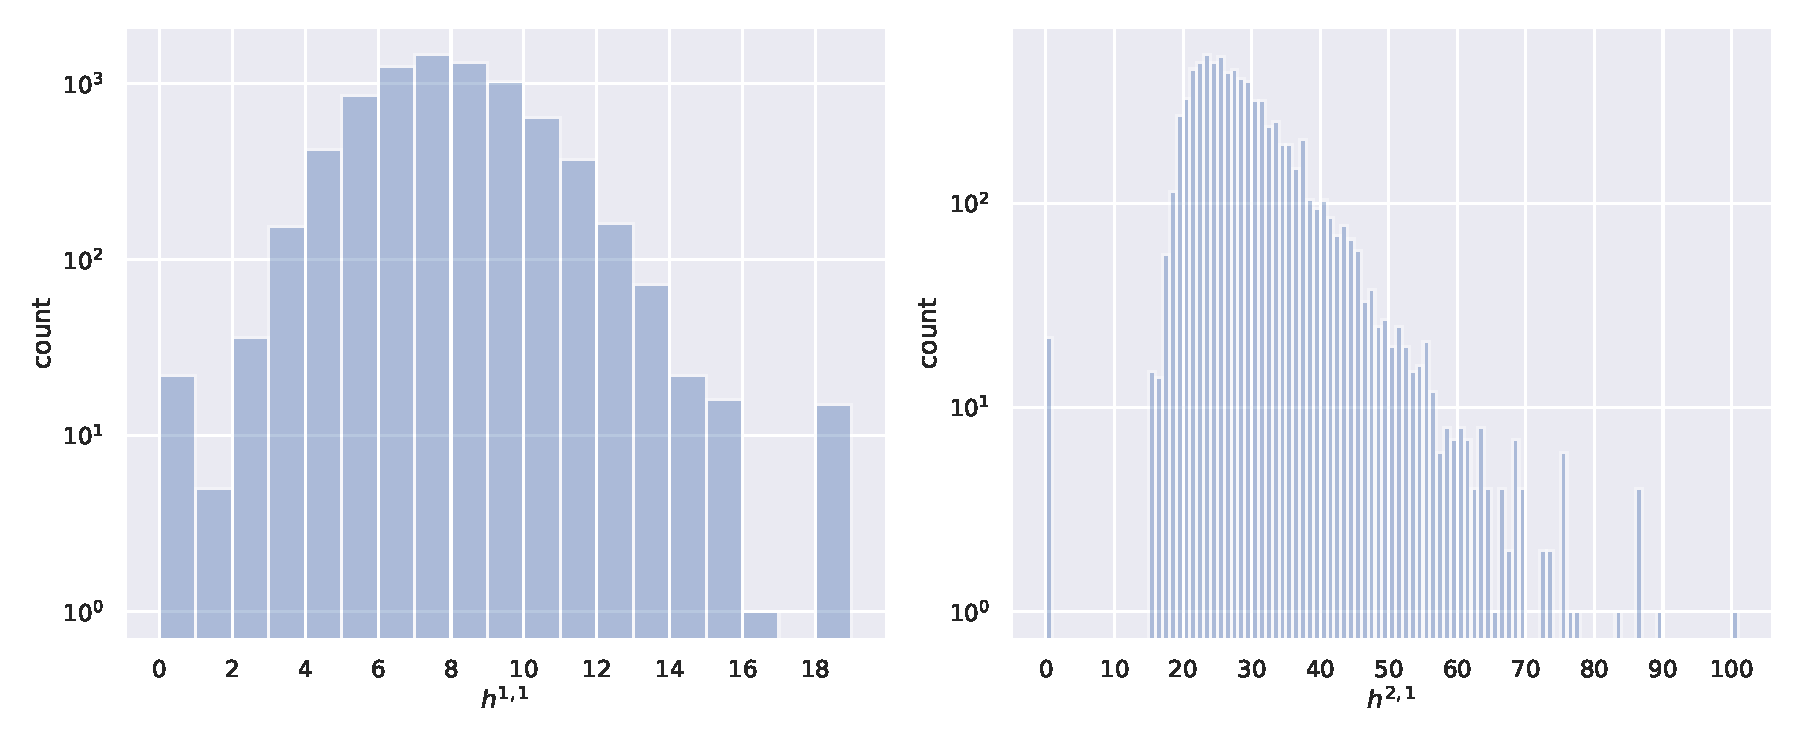
\includegraphics[width=\linewidth, trim={0 0.45in 6in 0}, clip]{img/label-distribution_orig}
    \caption{\hodge{1}{1}}
    \label{fig:data:hist-h11}
  \end{subfigure}
  \hfill
  \begin{subfigure}[c]{.45\linewidth}
    \centering
    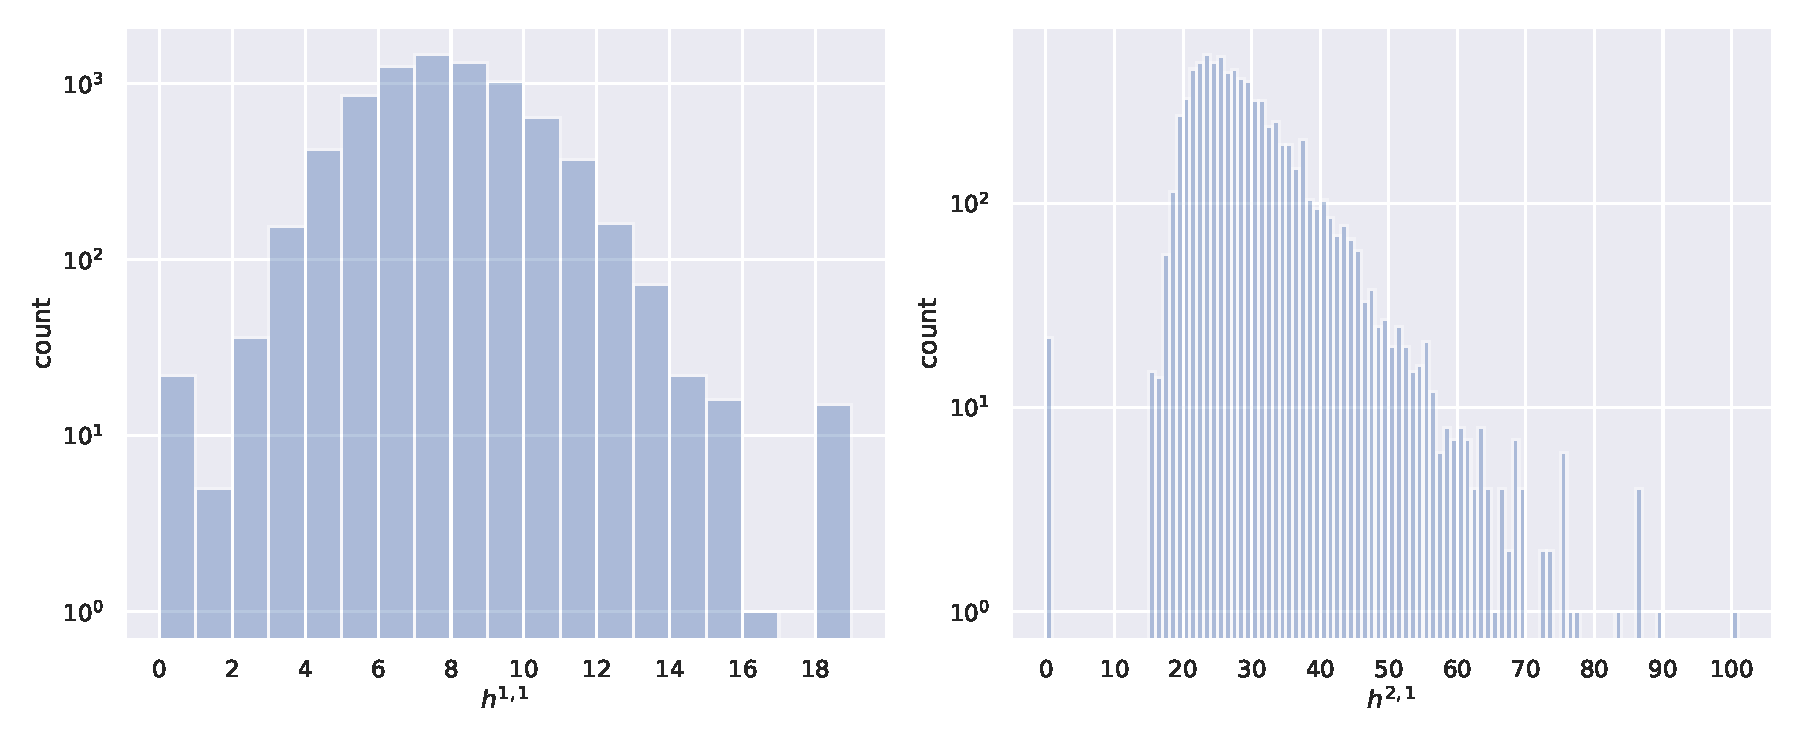
\includegraphics[width=\linewidth, trim={6in 0.45in 0 0}, clip]{img/label-distribution_orig}
    \caption{\hodge{2}{1}}
    \label{fig:data:hist-h21}
  \end{subfigure}
  \caption{Distribution of the Hodge numbers (log scale).}
  \label{fig:data:hist-hodge}
\end{figure}

The configuration matrix completely encodes the information of the \cicy and all topological quantities can be derived from it.
However the computations are involved and there is often no closed-form expression.
This situation is typical in algebraic geometry and it can be even worse for some problems, in the sense that it is not even known how to compute the desired quantity (e.g. the metric of \cy manifolds).
For these reasons it is interesting to study how to retrieve these properties using \ml algorithms.
In what follows we focus on the prediction of the Hodge numbers.
To provide a good test case for the use of \ml in context where the mathematical theory is not completely understood, we make no use of known formulas.


% vim: ft=tex


%---- APPENDIX
\appendix

%---- BIBLIOGRAPHY
\printbibliography[heading=bibintoc]

\end{document}

% vim: ft=tex
